\documentclass[a4paper,onecolumn,oneside,12pt,wide,floatssmall]{mwrep}
\usepackage{algorithm}
\usepackage{algpseudocode}
\usepackage{amsmath}
\usepackage{amsfonts}
\usepackage{amssymb}
\usepackage{amsthm}
\usepackage{float}
\usepackage{geometry}
\usepackage{listings}
\usepackage[pdftex]{color,graphicx}
\usepackage{polski}
\usepackage[pdftex, bookmarks=false]{hyperref}
\usepackage[table]{xcolor}
\usepackage{tikz}
\usepackage[T1]{fontenc}
\usepackage[utf8x]{inputenc}
\usepackage[sort, compress]{cite}
\makeatletter\renewcommand{\ALG@name}{Algorytm}

% interlinia 1,5
\linespread{1.3}

\newcommand{\norm}[1]{\lVert#1\rVert}
\def\url#1{{ \tt #1}}
\def\C{{\rm C}\,}
\def\E{{\rm E}\,}
\def\sgn{{\rm sgn}\,}

% marginesy
\textwidth\paperwidth
\advance\textwidth -55mm
\oddsidemargin-0.9in
\advance\oddsidemargin 33mm
\evensidemargin-0.9in
\advance\evensidemargin 33mm
\topmargin -1in
\advance\topmargin 25mm
\setlength\textheight{45\baselineskip}
\addtolength\textheight{\topskip}
\marginparwidth15mm

\clubpenalty=10000 % to kara za sierotki
\widowpenalty=10000 % nie pozostawia wdów
\brokenpenalty=10000 % nie dzieli wyrazów pomiędzy stronami
\sloppy

\tolerance4500
\pretolerance250
\hfuzz=1.5pt
\hbadness1450

% ŻYWA PAGINA
\renewcommand{\chaptermark}[1]{\markboth{\scshape\small\bfseries \
#1}{\small\bfseries \ #1}}
\renewcommand{\sectionmark}[1]{\markboth{\scshape\small\bfseries\thesection.\
#1}{\small\bfseries\thesection.\ #1}}
\newcommand{\headrulewidth}{0.5pt}
\newcommand{\footrulewidth}{0.pt}
\pagestyle{uheadings}

\theoremstyle{definition}
\newtheorem{defn}{Definicja}[section]
\newtheorem{conj}{Teza}[section]
\newtheorem{conjmain}{Teza}
\newtheorem{exmp}{Przykład}[section]

\theoremstyle{plain}% default
\newtheorem{thm}{Twierdzenie}[section]
\newtheorem{lem}[thm]{Lemat}
\newtheorem{prop}[thm]{Hipoteza}
\newtheorem*{cor}{Wniosek}

\theoremstyle{remark}
\newtheorem*{rem}{Uwaga}
\newtheorem*{note}{Uwaga}
\newtheorem{case}{Przypadek}

\definecolor{ListingBackground}{rgb}{0.95,0.95,0.95}

\begin{document}

\renewcommand*\lstlistingname{Wydruk}
\renewcommand*\lstlistlistingname{Spis wydruków}

\pagenumbering{roman}
\renewcommand{\baselinestretch}{1.0}
\raggedbottom
\begin{titlepage}
    % Strona tytułowa
    \vbox to\textheight{\hyphenpenalty=10000
    \begin{center}
	\begin{tabular}{p{107mm} p{9cm}}
	    \begin{minipage}{9cm}
	      \begin{center}
	      Politechnika Warszawska \\
	      Wydział Elektroniki i~Technik Informacyjnych \\
	      Instytut Informatyki
	      \end{center}
	    \end{minipage}
	    &
	    \begin{minipage}{8cm}
	    \begin{flushleft}
	     \footnotesize
	      Rok akademicki 2013/2014
	    \vspace*{2.75\baselineskip}
	    \end{flushleft}
	    \end{minipage} \\
	\end{tabular}
	\vspace*{3.75\baselineskip}
	\par\vspace{\smallskipamount}
	\vspace*{2\baselineskip}{\LARGE Praca dyplomowa magisterska\par}
	\vspace{3\baselineskip}{\LARGE\strut Adam Stelmaszczyk\par}
	\vspace*{2\baselineskip}{\huge\bfseries DE/mid -- nowy wariant algorytmu ewolucji różnicowej wykorzystujący punkt środkowy populacji\par}

	\vspace*{2\baselineskip}
	\hfill\mbox{}\par\vspace*{\baselineskip}\noindent
	\begin{tabular}[b]{@{}p{3cm}@{\ }l@{}}
	    {\large\hfill } & {\large }
	\end{tabular}
	\hfill
	\begin{tabular}[b]{@{}l@{}}
	Opiekun pracy: \\[\smallskipamount]
	{\large prof. nzw. dr hab. Jarosław Arabas}
	\end{tabular}\par
	\vspace*{2\baselineskip}
    \begin{tabular}{p{\textwidth}}
    \begin{flushleft}
	\begin{minipage}{7cm}
	Ocena \dotfill
	\par\vspace{1.6\baselineskip}
	\dotfill
	\par\noindent
	\centerline{\footnotesize Podpis Przewodniczącego} \par
	\centerline{\footnotesize Komisji Egzaminu Dyplomowego}\par
	\end{minipage}
    \end{flushleft}
    \end{tabular}
    \end{center}}

    % Życiorys
    \newpage\thispagestyle{empty}
    \begin{tabular}{p{5cm} p{12cm}}
    \begin{minipage}{5cm}
    \center
    
\includegraphics[height=6.5cm,width=4.5cm]{img/foto.jpg}
    \end{minipage}
    &
    \begin{minipage}{12cm}
    \begin{flushleft}
    \par\noindent\vspace{1\baselineskip}
    \begin{tabular}[h]{l l}
    {\normalsize\it Specjalność:} & \normalsize Inżynieria Systemów Informacyjnych 
    \end{tabular}
    \par\noindent\vspace{1\baselineskip}
    \begin{tabular}[h]{l l}
    {\normalsize\it Data urodzenia:} & {\normalsize 12 stycznia 1990~r.}
    \end{tabular}
    \par\noindent\vspace{1\baselineskip}
    \begin{tabular}[h]{l l}
    {\normalsize\it Data rozpoczęcia studiów:} & {\normalsize 1 października 2009 r.}
    \end{tabular}
    \par\noindent\vspace{1\baselineskip}
    \end{flushleft}
    \end{minipage}
    \end{tabular}
    \vspace*{1\baselineskip}
    \begin{center}
	{\large\bfseries Życiorys}\par\bigskip
    \end{center}

    \indent
Urodziłem się 12 stycznia 1990 roku w Piotrkowie Trybunalskim. Ukończyłem Szkołę Podstawową
nr 33, Gimnazjum nr 11 oraz Liceum Ogólnokształcące im. Jana Kochanowskiego w Warszawie, gdzie
uczęszczałem do klasy o profilu matematyczno--fizyczno--informatycznym.
W październiku 2009 roku rozpocząłem studia na Wydziale Elektroniki i Technik Informacyjnych
Politechniki Warszawskiej na kierunku Informatyka. W lutym 2013 roku uzyskałem tytuł inżyniera.

    \par
    \vspace{3\baselineskip}
    \hfill\parbox{15em}{{\small\dotfill}\\[-.3ex]
    \centerline{\footnotesize podpis studenta}}\par
    \vspace{2\baselineskip}
    \begin{center}
 	{\large\bfseries Egzamin dyplomowy} \par\bigskip
    \end{center}
    \par\noindent\vspace{1\baselineskip}
    Złożył egzamin dyplomowy w dn. \dotfill
    \par\noindent\vspace{1\baselineskip}
    Z wynikiem \dotfill
    \par\noindent\vspace{1\baselineskip}
    Ogólny wynik studiów \dotfill
    \par\noindent\vspace{1\baselineskip}
    Dodatkowe wnioski i uwagi Komisji \dotfill
  
    % Streszczenie
    \newpage\thispagestyle{empty}
    \vspace*{2\baselineskip}
    \begin{center}
	{\large\bfseries Streszczenie}\par\bigskip
    \end{center}

    {\itshape
W pracy przeanalizowano działanie znanych wariantów algorytmu ewolucji różnicowej~--~DE/rand
oraz DE/best. W celu poprawienia wyników zaproponowano nowy wariant nazwany DE/mid. 
Żeby porównanie jakości algorytmów było sprawiedliwe, każdemu z wariantów ustalono taki sam zasięg
mutacji poprzez dobranie odpowiedniego współczynnika skalującego.
Na podstawie przeprowadzonych testów stwierdzono poprawę jakości uzyskiwanych wyników na 6 z 7 
wielowymiarowych funkcji testowych z zestawu BBOB 2013.}
    \vspace*{1\baselineskip}

    \noindent{\bf Słowa kluczowe}: {\itshape ewolucja różnicowa, algorytm ewolucyjny, genetyczny, optymalizacja globalna}
    \par
    \vspace{4\baselineskip}
    \begin{center}
	{\large\bfseries Abstract}\par\bigskip
    \end{center}
    \noindent{\bf Title}: {\itshape DE/mid -- new variant of differential evolution algorithm using the midpoint of the population}\par
    \vspace*{1\baselineskip}
    {\itshape
This thesis analyzes behaviour of known differential evolution variants -- DE/rand and DE/best.
In order to achieve better performance, new variant named DE/mid has been introduced.
To ensure a fair comparison between algorithms, mutation of every algorithm variant had exactly
the same range. 
Tests indicated improvement of results quality on 6 out of 7 high-dimensional
testing functions from BBOB 2013 testbed.}
    \vspace*{1\baselineskip}

    \noindent{\bf Key words}: {\itshape differential evolution, evolutionary, genetic algorithm, global optimization
}

\end{titlepage}

\tableofcontents

\newpage
\pagenumbering{arabic}
\setcounter{page}{1}

\chapter{Wstęp}

Optymalizacja globalna polega na znalezieniu ekstremum 
globalnego (minimum bądź maksimum) pewnej funkcji, zwanej funkcją celu. 
Funkcja ta jest ,,czarną skrzynką'', tzn. nie można
zakładać znajomości tej funkcji podczas projektowania algorytmu optymalizacji.
W związku z~tym analityczne wyznaczenie ekstremów nie jest możliwe. W przypadku 
skomplikowanych funkcji znalezienie dokładnego optimum może być bardzo czasochłonne, 
a w praktyce wręcz niewykonalne. Wówczas celem jest znalezienie możliwie najlepszego rozwiązania
suboptymalnego. Algorytm optymalizujący wybiera pewne rozwiązanie, następnie poddaje to rozwiązanie 
ocenie przez funkcję oceniającą, w wyniku czego otrzymuje liczbową wartość (jakość, dobroć) 
podanego rozwiązania. 
Proces optymalizacji przebiega w sposób iteracyjny, tzn. nowe rozwiązania powstają w~wyniku przetworzenia
poprzednich.

Przykładowo, ,,czarną skrzynką'' może być program (symulator), który, po podaniu 
parametrów na wejście, przeprowadza jeden eksperyment i zwraca np. liczbę watów wygenerowanych
przez panele słoneczne. Parametrami wejściowymi mogą być kąty nachylenia i prędkości obrotu paneli. 
Panele te umieszczone są na sztucznym satelicie, który krąży po orbicie ziemskiej.
Przez to niektóre panele rzucają cień na inne, jeśli są źle ustawione. Panele również nie mogą być 
zbyt długo wystawione na działanie promieni słonecznych, ponieważ może dojść do ich uszkodzenia. 
To wprowadza kłopotliwe ograniczenia w przestrzeni przeszukiwań.
Symulator przeprowadza kosztowne obliczenia, żeby zwrócić całkowitą liczbę watów wygerenowanych
przez panele w ciągu pełnego obiegu satelity wokół Ziemi. Zadanie optymalizacji polega w tym przypadku na
doborze takich parametrów wejściowych, które powodują wygenerowanie jak największej liczby watów
przez wszystkie panele.

Ewolucja różnicowa (ang. differential evolution, DE) jest algorytmem przeznaczonym 
do optymalizacji globalnej w przestrzeniach ciągłych \cite{storn}.
Algorytm ten może mieć wiele postaci (wariantów), w zależności od używanych
operatorów genetycznych -- selekcji, mutacji oraz krzyżowania. 
Ewolucja różnicowa jest atrakcyjnym algorytmem ze względu na nieskomplikowaną
definicję i małą liczbę parametrów. Jednocześnie jej efektywność jest porównywalna do innych metod
optymalizacji startujących w~konkursach typu BBOB \cite{setup} czy CEC \cite{cec}.

\section{Cel pracy}

Celem pracy była poprawa efektywności algorytmu ewolucji różnicowej.
Wiązało się to ze szczegółową analizą i przetestowaniem istniejących wariantów algorytmu,
a~następnie zapronowaniem lepszej metody. 
Skoncentrowano się na odpowiednim doborze operatora selekcji.
Nowy wariant ewolucji różnicowej, nazwany DE/mid, został porównany 
do dwóch znanych odmian -- DE/rand oraz DE/best. 
Wyniki eksperymentów wskazały na znaczną przewagę DE/mid na 6 z 7 wielowymiarowych 
funkcji testowych.

\section{Układ pracy}

Rozdział pierwszy stanowi wprowadzenie do tematu pracy, definiując jej cel oraz podstawowe pojęcia.
W rozdziale drugim wyjaśniono podstawy działania algorytmów ewolucyjnych. 
Następnie opisano schemat ewolucji różnicowej, a także trzy operatory genetyczne -- selekcję,
mutację oraz krzyżowanie. 
W rozdziale trzecim zaprezentowano nowy wariant ewolucji różnicowej nazwanej DE/mid. 
W części tej dokonano również analizy macierzy kowariancji rozkładu mutantów dla różnych wariantów ewolucji
różnicowej. Na tej podstawie wyprowadzono 
wzory na współczynniki skalujące -- istotny parametr algorytmu ewolucji różnicowej mający bezpośredni
wpływ na zasięg mutacji. 
W~rodziale czwartym opisano metodykę testowania, jakich dokładnie funkcji testowych 
używano.
Wyjaśniono również w jaki sposób testy zostały 
zaimplementowane oraz jak została sprawdzona ich poprawność. Na zakończenie rodziału opisano
metodę porównywania wyników eksperymentów -- zwrócono uwagę na testy istotności 
statystycznej, dystrybuanty empiryczne oraz liczbę osobników poza zbiorem dopuszczalnym.
W rozdziale piątym zaprezentowano w sposób zbiorczy wyniki wszystkich eksperymentów,
przedstawiono również wnioski z nich płynące. 
Pracę kończy podsumowanie oraz wskazanie możliwych kierunków dalszego rozwoju.

\section{Słownik pojęć i oznaczeń}

\begin{itemize}
 \item[] Osobnik, punkt, wektor, rozwiązanie -- podstawowy element przestrzeni przeszukiwań, 
przetwarzany przez algorytm ewolucji różnicowej
 \item[] Populacja -- zbiór osobników, przetwarzany w pojedynczej iteracji algorytmu
 \item[] DE (ang. Differential Evolution) -- ewolucja różnicowa
 \item[] DE/rand -- klasyczny wariant DE wybierający losowy punkt w selekcji
 \item[] DE/best -- klasyczny wariant DE wybierający najlepszy punkt w selekcji
 \item[] DE/mid -- zaproponowany w pracy wariant DE wybierający punkt środkowy w~selekcji
 \item[] DE/X/k/Z -- skrócony zapis nazwy wariantu DE, X oznacza rodzaj selekcji (np. rand, best, mid), k oznacza liczbę wektorów różnicowych stosowanych
w mutacji (domyślnie 1), zaś Z to rodzaj krzyżowania (domyślnie bin -- dwumianowe).
 \item[] BBOB (ang. Black-Box Optimization Benchmarking) -- nazwa warsztatów poświęconych testowaniu algorytmów optymalizacji. 
Warsztaty te odbywały się w latach 2009, 2010, 2012 oraz 2013. Zmieniały się algorytmy startujące w konkursie, nie zmieniał
się sposób ich testowania (opisany w rozdziale \ref{sec:zestaw}).
 \item[] $k$ -- liczba wektorów różnicowych używanych w mutacji
 \item[] $\mu$ -- liczba osobników w populacji
 \item[] $D$ -- liczba cech osobnika, również wymiar optymalizowanej funkcji
 \item[] $P^t$ -- populacja o numerze $t$
 \item[] $P_i^t$ -- osobnik o indeksie $i$ w populacji $P^t$
 \item[] $O^t$ -- populacja potomków u numerze $t$
 \item[] $O_i^t$ -- osobnik o indeksie i w populacji potomków $O^t$
 \item[] $v_i$ -- punkt wybrany w selekcji w iteracji $i$
 \item[] $u_i$ -- mutant w iteracji $i$
 \item[] $o_i$ -- potomek po krzyżowaniu w iteracji $i$
 \item[] $F$ (ang. Factor) -- współczynnik skalujący, parametr ewolucji różnicowej sterujący zasięgiem mutacji
 \item[] $CR$ (ang. Crossover Rate) -- prawdopodobieństwo krzyżowania, parametr algorytmów ewolucyjnych sterujący częstością krzyżowań
 \item[] $f$ -- funkcja celu, przystosowania, oceny, optymalizowana funkcja, funkcja testowa
 \item[] $f_\text{opt}$ -- optymalna wartość $f$, tzn. minimum podczas minimalizacji lub maksimum podczas maksymalizacji
 \item[] $\C[u]$ -- macierz kowariancji rozkładu zmiennej losowej $u$
\end{itemize}

\chapter{Ewolucja różnicowa}

\section{Algorytm ewolucyjny}

Algorytmy ewolucyjne to rodzaj algorytmów, w których wykorzystywane są operatory genetyczne (selekcja,
mutacja, krzyżowanie) na zbiorach punktów w przestrzeni przeszukiwań nazywanych populacjami \cite{jarabas}. 
Celem działania algorytmu jest
wyznaczenie ektremum globalnego (minium bądź maksimum) optymalizowanej funkcji.
Zasadę działania typowego algorytmu ewolucyjnego przedstawiano na listingu \ref{algorithm:ea}.

\begin{algorithm}[H]
\caption{Algorytm ewolucyjny}
\label{algorithm:ea}
\begin{algorithmic}[1]
\State Inicjalizacja parametrów $CR, \mu$
\State Inicjalizacja populacji początkowej $P^1 \gets \{P^1_1, P^1_2, \ldots, P^1_{\mu}\}$
\State $t \gets 1$
\While{kryterium stopu nie zostało spełnione}
  \ForAll{$i \in \{ 1, 2, \ldots, \mu \}$}
    \If{$\mathcal{U}(0, 1) < CR$}
      \State $O^t_i \gets$ mutacja(krzy{\.z}owanie(selekcja($P(t)$), selekcja($P(t)$)))
    \Else
      \State $O^t_i \gets$ mutacja(selekcja($P(t)$))
    \EndIf
  \EndFor
  \State $P^{t+1} \gets$ sukcesja$(P^t, O^t)$
  \State $t \gets t+1$
\EndWhile
\end{algorithmic}
\end{algorithm}

$\mathcal{U}(0, 1)$ to realizacja zmiennej losowej o rozkładzie jednostajnym na przedziale od 0 do 1.
Algorytm ewolucyjny w podstawowej postaci ma trzy parametry wejściowe.
Są nimi: $CR$~--~prawdopodobieństwo krzyżowania, $\mu$ -- liczba osobników w populacji
oraz $F$ -- współczynnik skalujący wykorzystywany w mutacji.
Po nadaniu wartości początkowych parametrom, następuja inicjalizacja populacji początkowej. 
Jeśli zupełnie nie wiadomo, gdzie może znajdować się poszukiwane optimum, 
populację początkową generuje się w sposób losowy z rozkładem jednostajnym w zbiorze dopuszczalnym.

Po inicjalizacji populacji początkowej następuje główna pętla programu. 
Wykonywana jest ona dopóty, dopóki nie zajdzie tzw. kryterium stopu. 
Kryterium stopu może być np. maksymalna liczba iteracji lub wywołań funkcji oceny.
Algorytm można zatrzymać również wtedy, gdy znalezione rozwiązanie jest zadowalające. 

W głównej pętli programu przetwarzana jest bieżąca populacja. 
Wykonywana jest kolejna pętla, tym razem iterująca kolejno po wszystkich osobnikach 
(rozwiązaniach) z bieżącej populacji. W niej losowana jest liczba od 0 do 1 i jeśli jest ona mniejsza
od ustalonego $CR$ -- dokonywana jest selekcja dwóch punktów, ich krzyżowanie, a następnie mutacja.
W przeciwnim przypadku krzyżowanie jest pomijane.
Po wygenerowaniu populacji potomków $O^t$ następuje sukcesja, czyli wybór punktów, które przechodzą
do następnej populacji $P^{t+1}$. Zwiększany jest licznik populacji (czasu) $t$,
sprawdzane jest kryterium stopu i jeśli nie jest spełnione --
wykonywana jest kolejna pętla.
 
Kolejnym problemem jest dobór parametrów dla algorytmu ewolucyjnego. 
Istnieją pewne porady, np. stosowana w tej pracy reguła $\mu = 10D$, 
jednak w ogólnym przypadku nie wiadomo jaki rozmiar populacji czy jakie prawdopodobieństwo
krzyżowania $CR$ sprawdzi się najlepiej. Duży problem również stanowi dobór parametrów dla mutacji.
Z pomocą przychodzą
metody samoadaptacji, które same dostrajają parametry algorytmu w zależności od stanu w jakim się
znajdują, np. w~zależności od zawartości populacji \cite{brest}.
Ewolucja różnicowa radzi sobie z problemem doboru parametrów właśnie dzięki pewnemu rodzajowi
samoadaptacji.

\section{Algorytm ewolucji różnicowej}

Ewolucja różnicowa jest algorytmem ewolucyjnym służącym do optymalizacji
w przestrzeniach ciągłych zaproponowanym w 1995 roku. \cite{storn} Sposób działania algorytmu
przedstawiono na listingu \ref{algorithm:de}.

\usetikzlibrary{decorations.pathreplacing,calc}
\newcommand{\tikzmark}[1]{\tikz[overlay,remember picture] \node (#1) {};}

\newcommand*{\AddNote}[4]{%
    \begin{tikzpicture}[overlay, remember picture]
        \draw [decoration={brace,amplitude=0.5em},decorate,thick]
            ($(#3)!(#1.north)!($(#3)-(0,1)$)$) --  
            ($(#3)!(#2.south)!($(#3)-(0,1)$)$)
                node [align=center, text width=2.5cm, pos=0.5, anchor=west] {#4};
    \end{tikzpicture}
}%

\begin{algorithm}[H]
\caption{Ewolucja różnicowa}
\label{algorithm:de}
\begin{algorithmic}[1]
\State Inicjalizacja parametrów $CR, F, \mu$
\State Inicjalizacja populacji początkowej $P^1 \gets \{P^1_1, P^1_2, \ldots, P^1_\mu\}$
\State $t \gets 1$
\While{kryterium stopu nie zostało spełnione}
  \ForAll{$i \in \{ 1, 2, \ldots, \mu \}$}
    \State $v_i \gets$ selekcja$(P^t_i)$
    \State $u_i \gets$ mutacja$(v_i, P^t_i, F)$ 
    \State $o_i \gets$ krzy{\.z}owanie$(u_i, P_i^t, CR)$    
    \If{$f(o_i) \le f(P_i^t)$}  \tikzmark{top} \tikzmark{right} 
      \State $P_i^{t+1} \gets o_i$     
    \Else 
      \State $P_i^{t+1} \gets P_i^{t}$
    \EndIf \tikzmark{bottom}
  \EndFor
\EndWhile \\
\Return arg min$_i f(P^t_i)$ \AddNote{top}{bottom}{right}{~~sukcesja}
\end{algorithmic}
\end{algorithm}

Bardzo istotną różnicą pomiędzy ewolucją różnicową a typowym algorytmem ewolucyjnym jest sposób mutacji.
W ewolucji różnicowej punkty są od siebie odejmowane, w wyniku czego powstają wektory różnicowe. 
Następnie mutowane punkty są przesuwane o te wektory. Natomiast w typowym algorytmie ewolucyjnym
odejmowanie nie występuje -- mutacja polega na dodawaniu losowego wektora do mutowanych punktów.
Kolejność wykonywania operatorów mutacji oraz krzyżowania w~ewolucji różnicowej
jest również inna niż w typowym algorytmie ewolucyjnym.
W algorytmie ewolucyjnym najpierw wykonywane jest krzyżowanie, potem mutacja.
W ewolucji różnicowej -- na odwrót.
Kolejną różnicą jest konkretyzacja operatora sukcesji. W ewolucji różnicowej, po wygenerowaniu potomka
$o_i$ jest on od razu porównywany ze swoim rodzicem. Jeśli okaże się lepszy -- zastępuje go
w~kolejnej populacji. Powoduje to silny nacisk selektywny -- dalej przechodzą jedynie dzieci
lepiej przystosowane od swoich rodziców.

W tej pracy stosowany jest zapis nazwy algorytmu w postaci \mbox{DE/X/k/Z},
gdzie X oznacza rodzaj selekcji (np. rand, best, mid), k oznacza liczbę wektorów różnicowych stosowanych
w mutacji (domyślnie 1), zaś Z to rodzaj krzyżowania (domyślnie bin -- dwumianowe).

\subsection{Selekcja}

Operator selekcji na wejściu otrzymuje bieżącą populację i zwraca jedno rozwiązanie.
W tej pracy zwrócono szczególną uwagę na właściwy dobór tego operatora.
Skrót DE/rand oznacza ewolucję różnicową z losowym typem selekcji, tzn. wybierany jest jeden
losowy punkt z całej populacji zgodnie z rozkładem jednostajnym:
W wariancie DE/best wybierany jest punkt najlepszy. Zaproponowany w tej pracy DE/mid wybiera
punkt środkowy populacji. 
DE/rand-to-best stanowi połączenie DE/rand oraz DE/best -- punkt wybierany w selekcji $v_i$ 
to liniowa kombinacja punktu najlepszego $x_*$ oraz losowego $x_{i_1}$ z wagami $\lambda$ oraz $(1 - \lambda)$:

$$ v_i = \lambda x_* + (1 - \lambda)x_{i_1} $$

gdzie $\lambda \in (0, 1)$. Wariant DE/current-to-best jest podobny DE/rand-to-best, z~tym, że zamiast punktu
losowego występuje punkt bieżący $x_i$.
Natomiast w DE/current-to-rand punktem wybieranym w selekcji jest liniowa kombinacja 
punktu bieżącego $x_i$ oraz losowego $x_{i_1}$ \cite{zaharie}.

\subsection{Mutacja}

Operator mutacji na wejściu otrzymuje jedno rozwiązanie i zwraca również jedno.
Jako trzeci człon skróconej nazwy algorytmu
podawana jest liczba wektorów różnicowych używanych w mutacji -- $k$.
Np. DE/rand/1 oznacza losową selekcję z jednym wektorem różnicowym w mutacji.
Ten podstawowy wariant algorytmu nazywany jest również ,,klasyczną'' ewolucją różnicową. 

\subsection{Krzyżowanie}
\label{sec:krzyzowanie}

Operator krzyżowania na wejściu otrzymuje dwa rozwiązania rodzicielskie, a zwraca jedno potomne. 
W ewolucji różnicowej jednym z rodziców jest mutant. 
Często wykorzystywanym rodzajem krzyżowania jest krzyżowanie wymieniające, w którym 
część rozwiązania jest brana od jednego z rodziców, a pozostała część od drugiego. 
Krzyżowanie wymieniające ma dwie odmiany -- bin (ang. binomial -- dwumianowe) oraz 
exp (ang. exponential -- wykładnicze). Sposób działania krzyżowania dwumianowego przedstawiono na listingu \ref{algorithm:bin}.

\begin{algorithm}[H]
\caption{Krzyżowanie dwumianowe (bin)}
\label{algorithm:bin}
\begin{algorithmic}[1]
\State Wejście: dwa rozwiązania rodzicielskie $x_1, x_2$ 
\State $o \gets x_1$
\ForAll{$d \in \{ 1, 2, \ldots, D \}$}
  \If{$\mathcal{U}(0, 1) < CR$} 
    \State $o[d] \gets x_2[d]$     
  \EndIf 
\EndFor \\
\Return $o$
\end{algorithmic}
\end{algorithm}

$\mathcal{U}(0, 1)$ to realizacja zmiennej losowej o rozkładzie jednostajnym na przedziale od 0 do 1.
$CR$ (ang. Crossover Rate) to sparametryzowane prawdopodobieństwo krzyżowania. 
Sposób działania krzyżowania wykładniczego przedstawiono na listingu \ref{algorithm:exp}.

\begin{algorithm}[H]
\caption{Krzyżowanie wykładnicze (exp)}
\label{algorithm:exp}
\begin{algorithmic}[1]
\State Wejście: dwa rozwiązania rodzicielskie $x_1, x_2$ 
\State $o \gets x_1$
\State $d \gets 1$
\While{$d \leq D$ \textbf{and} $\mathcal{U}(0, 1) < CR$}
    \State $o[d] \gets x_2[d]$ 
    \State $d \gets d + 1$
\EndWhile \\
\Return $o$
\end{algorithmic}
\end{algorithm}

W tej pracy w każdym z wariantów ewolucji różnicowej stosowano krzyżowanie dwumianowe (bin).

\subsection{Inne modyfikacje ewolucji różnicowej}

Można wprowadzić olbrzymią liczbę modyfikacji do podstawowego algorytmu ewolucji różnicowej.
Oprócz zmian w podstawowych operatorach genetycznych, możliwe jest również dodawanie reguł adaptacyjnych.
Przykładami mogą być algorytmy SaDE oraz jDE wykorzystujące metody losowego wyboru
wartości parametrów \cite{brest}. Istnieją również podejścia hybrydowe, np. w algorytmach JADE \cite{jade} oraz 
DEPSO \cite{depso} wykorzystano elementy znane w algorytmach optymalizacji rojem cząstek (ang. PSO -- Particle Swarm Optimization).

\chapter{Algorytm DE/mid -- nowy wariant ewolucji różnicowej}
\label{chap:de_mid}

W tym rozdziale przeanalizowano rozkłady mutantów różnych wariantów ewolucji różnicowej.
Dla ustalenia tego samego zasięgu mutacji kluczowe było wyprowadzenie odpowiednych współczynników skalujących
dla każdego z wariantów DE. Następnie przedstawiono nowy wariant ewolucji różnicowej nazwanej DE/mid.

\section{Analiza macierzy kowariancji dla podstawowych wariantów DE}

W poniższych podrozdziałach przedstawiono operatory mutacji dla DE/rand/k, DE/best/k, DE/mid/k 
oraz wyprowadzono wzory na współczynniki skalujące $F$. We wzorach, dla zwiększenia
czytelności, pomijano indeks górny $t$ dla populacji, np. stosowano zapis $P_{i_1}$ 
zamiast $P_{i_1}^t$.

\subsection{DE/rand}
\label{chap:de_rand} 

W DE/rand/1, $i$-ty mutant w populacji $P$~o~$\mu$~osobnikach powstaje w następujący sposób 
\cite{decomposition}:
\begin{equation} \label{eq:derand1}
u_i = P_{i_1} + F(P_{i_2} - P_{i_3})
\end{equation}

$i_1, i_2, i_3$ to indeksy wylosowane zgodnie z rozkładem jednostajnym ze zbioru \\ 
$\{1, 2, \dots, \mu\}$. Zatem $P_{i_1}, P_{i_2}, P_{i_3}$ to rozwiązania wylosowane zgodnie z 
rozkładem jednostajnym z populacji $P$.
$F\in\mathbb{R_+}$ to współczynnik skalujący zasięg mutacji. 

DE/rand/1 można uogólnić na DE/rand/k, w którym dodawanych jest
$k \in \mathbb{N}$ wektorów różnicowych:
\begin{equation} \label{eq:derand}
u_i' = P_{i_1} + F_k\sum\limits_{j=1}^k (P_{i_{2j}} - P_{i_{2j+1}})
\end{equation}

Podobnie jak poprzednio, $i_1, i_2, \dots i_{2k+1}$ to indeksy wylosowane zgodnie z rozkładem jednostajnym ze zbioru 
$\{1, 2, \dots, \mu\}$. Zatem $P_{i_1}, P_{i_2}, \dots, P_{2k+1}$ to rozwiązania wylosowane zgodnie z rozkładem 
jednostajnym z populacji $P$. $F_k\in\mathbb{R_+}$ to współczynnik skalujący dla DE/rand/k. 

Żeby zasięg mutacji nie zmieniał się wraz ze wzrostem $k$, 
macierz kowariancji mutanta $u_i'$ musi być taka sama jak macierz kowariancji mutanta $u_i$.
Można to osiągnąć tak dobierając $F_k$, aby było spełnione równanie:
\begin{equation} \label{eq:kowariancje}
\C[u_i] = \C[u_i']
\end{equation}

$\C[u_i]$ jest macierzą kowariancji rozkładu zmiennej losowej $u_i$.
Rozwijając lewą stronę równania \eqref{eq:kowariancje} i korzystając z tego, że osobniki są niezależne od siebie:
\begin{align*}
\C[u_i] \overset{(\ref{eq:derand1})}{=} \C[P_{i_1} + F(P_{i_2} - P_{i_3})] = \C[P_{i_1}] + F^2(\C[P_{i_2}] + \C[P_{i_3}])
\end{align*}

Każdy osobnik ma taki sam rozkład prawdopodobieństwa. 
Macierz kowariancji punktów losowanych z $P$ ma teorytyczną wartość $\C[P]$,
równą empirycznej macierzy kowariancji populacji $P$.
Zatem dla DE/rand/1 macierz kowariancji mutanta wynosi:
\begin{equation} \label{eq:macierz_kow_mutanta}
\C[u_i] = \C[P] + F^2(\C[P] + \C[P]) = \C[P](2F^2 + 1)
\end{equation}

Rozwijając prawą stronę równania \eqref{eq:kowariancje}, w przypadku DE/rand/k macierz kowariancji mutanta wynosi:
\begin{equation}
\begin{align}
 \label{eq:macierz_kow_mutanta_prim}
\C[u_i'] \overset{(\ref{eq:derand})}{=} \C[P_{i_1} + F_k\sum\limits_{j=1}^k (P_{i_{2j}} - P_{i_{2j+1}})] 
&= \C[P_{i_1}] + F_k^2\C[\sum\limits_{j=1}^k (P_{i_{2j}} - P_{i_{2j+1}})] \\
&= \C[P_{i_1}] + F_k^2\C[\sum\limits_{j=2}^{2k+1} P_{i_{j}}] = \C[P](2kF_k^2 + 1)
\end{align}
\end{equation}

Przyrównując \eqref{eq:macierz_kow_mutanta} oraz \eqref{eq:macierz_kow_mutanta_prim}:
\begin{align*}
\C[P](2F^2 + 1) = \C[P](2kF_k^2 + 1)
\end{align*}

Przy założeniu, że $\C[P] \neq \textbf{0}$:
\begin{align*}
F^2 = kF_k^2
\end{align*}

Obie strony są nieujemne, więc ostatecznie:
\begin{align*}
F_k = \frac{F}{\sqrt{k}}
\end{align*}

Zatem, dla zachowania zasięgu mutacji, współczynik skalowania dla DE/rand/k powinien być  
$\sqrt{k}$ razy mniejszy od współczynnika skalowania dla DE/rand/1. Po wstawieniu powyższego wyniku
do \eqref{eq:derand}, wzór na mutanta dla DE/rand/k można zapisać nastepująco:

$$ u_i' = P_{i_1} + \frac{F}{\sqrt{k}}\sum\limits_{j=1}^k (P_{i_{2j}} - P_{i_{2j+1}}) $$

\subsection{DE/rand/$\infty$}
\label{sub:de_rand_inf}

Wariant DE/rand/$\infty$ został zaproponowany w \cite{decomposition} i nie jest wariantem klasycznym.
Zgodnie z centralnym twierdzeniem granicznym, część $\frac{1}{{\sqrt{k}}}\sum\limits_{j=1}^k (P_{i_{2j}} - P_{i_{2j+1}})$ 
zbiega według rozkładu do $\mathcal{N}(0, \C[P])$ gdy $k \to \infty$. 
Dzięki temu, równanie mutanta DE/rand/$\infty$ można zapisać jako:
\begin{align*}
u_i^\infty = P_{i_1} + F_\infty \cdot v_\infty
\end{align*}

gdzie $v_\infty \sim \mathcal{N}(0, \C[P])$. Współczynnik $F_\infty$ zapewniający
równość macierzy kowariancji dla wariantów DE/rand/1 oraz DE/rand/$\infty$
można wyznaczyć następująco:
\begin{align*}
\C[u_i^\infty] &= \C[u_i] \\
\C[P_{i_1} + F_\infty \cdot v_\infty] &= \C[P](2F^2 + 1) \\
\C[P] + \C[F_\infty \cdot v_\infty] &= \C[P](2F^2 + 1) \\
\C[F_\infty \cdot v_\infty] &= 2F^2\C[P] \\
F_\infty^2 \C[P] &= 2F^2\C[P] \\
F_\infty^2 &= 2F^2 \\
F_\infty &= \sqrt{2}F
\end{align*}

\subsection{DE/best}

W DE/best/k, $i$-ty mutant w populacji $P$~o~$\mu$~osobnikach powstaje w następujący sposób:
\begin{equation} \label{eq:debest}
u_i^* = P_* + F_*\sum\limits_{j=1}^k (P_{i_{2j}} - P_{i_{2j+1}})
\end{equation}

gdzie $P_*$ to najlepszy osobnik w populacji $P$. Formalnie:
\begin{equation} \label{eq:best_point}
P_* = \text{arg} \min_i f(P_i)
\end{equation}

Podobnie jak w przypadku DE/rand/k, $i_2, i_3, \dots i_{2k+1}$ to indeksy wylosowane zgodnie z rozkładem jednostajnym ze zbioru 
$\{1, 2, \dots, \mu\}$. $F_*\in\mathbb{R_+}$ to współczynnik skalujący dla DE/best/k. 

Żeby zasięg mutacji nie zmieniał się wraz ze wzrostem $k$, 
macierz kowariancji mutanta $u_i^*$ musi być taka sama jak macierz kowariancji mutanta $u_i$.
Można to osiągnąć tak dobierając $F_k$, aby było spełnione równanie:
\begin{equation} \label{eq:kowariancje_best}
\C[u_i] = \C[u_i^*]
\end{equation}

Rozwijając prawą stronę równania \eqref{eq:kowariancje_best},  macierz kowariancji mutanta dla DE/best/k wynosi:
\begin{equation}
\begin{align}
 \label{eq:macierz_kow_mutanta_star}
\C[u_i^*] &\overset{\eqref{eq:debest}}{=} \C[P_* + F_*\sum\limits_{j=1}^k (P_{i_{2j}} - P_{i_{2j+1}})] 
= \C[P_*] + F_*^2\C[\sum\limits_{j=1}^k (P_{i_{2j}} - P_{i_{2j+1}})] \\
&= \frac{1}{\mu}\C[P] + F_*^2\C[\sum\limits_{j=2}^{2k+1} P_{i_{j}}] = \C[P](2kF_*^2 + \frac{1}{\mu})
\end{align}
\end{equation}

Przyrównując \eqref{eq:macierz_kow_mutanta} oraz \eqref{eq:macierz_kow_mutanta_star}:
\begin{align*}
\C[P](2F^2 + 1) = \C[P](2kF_*^2 + \frac{1}{\mu})
\end{align*}

Przy założeniu, że $\C[P] \neq \textbf{0}$:
\begin{align*}
2F^2 + 1 &= 2kF_*^2 + \frac{1}{\mu} \\
F_*^2 &= \frac{2F^2 + 1 - \frac{1}{\mu}}{2k}
\end{align*}

Obie strony są nieujemne, więc ostatecznie:
\begin{align*}
F_* = \sqrt{\frac{2F^2 + 1 - \frac{1}{\mu}}{2k}}
\end{align*}

\subsection{DE/best/$\infty$}
\label{sub:de_rand_inf}

Przechodząc z $k$ do nieskończności, równanie mutanta DE/best/$\infty$ można zapisać jako:
\begin{align*}
u_i^{\infty^*} = P_* + F_{\infty_*} \cdot v_{\infty_*}
\end{align*}

gdzie $v_{\infty_*} \sim \mathcal{N}(0, \C[P])$. Współczynnik skalujący $F_{\infty_*}$ zapewniający
równość macierzy kowariancji dla wariantów DE/rand/1 oraz DE/best/$\infty$
można wyznaczyć następująco:
\begin{align*}
\C[u_i^{\infty^*}] &= \C[u_i] \\
\C[P_* + F_{\infty_*} \cdot v_{\infty_*}] &= \C[P](2F^2 + 1) \\
\C[P_*] + \C[F_{\infty_*} \cdot v_{\infty_*}] &= \C[P](2F^2 + 1) \\
\frac{\C[P]}{\mu} + F_{\infty_*}^2 \C[P] &= \C[P](2F^2 + 1) \\
F_{\infty_*} &= \sqrt{2F^2 + 1 - \frac{1}{\mu}}\\
\end{align*}

\section{Analiza rozkładu mutantów dla podstawowych wariantów DE}

\subsection{Symetria rozkładu mutantów}

W tym podrozdziale przyjęto przestrzeń o jednym wymiarze $x$.
Populację początkową przedstawiono na rysunku \ref{fig:sym_none}.
Są nią 4 punkty o wartościach $x$ równych kolejno $-0.5, 0, 0.5, 3$.
Punkty te dobrano specjalnie w taki sposób, aby można było zaobserwować asymetrię
rozkładu mutantów dla DE/rand/1 -- trzy pierwsze punkty znajdują się w grupie po lewej stronie, 
po prawej natomiast znajduje się tylko jeden punkt.
Współczynnik skalujący $F$ wynosił 1, dla uproszczenia.
Dla DE/best/1 przyjęto, że najlepszym punktem był punkt o $x = 0$.

\begin{figure}[H]
\centering
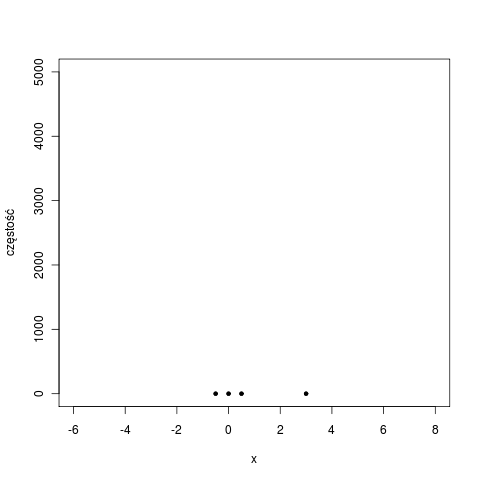
\includegraphics[width=.65\textwidth]{img/none}
\caption{6 punktów populacji początkowej} 
\label{fig:sym_none}
\end{figure}
Rysunek \ref{fig:sym_best} przedstawia histogram częstości występowania
mutantów (zaznaczonych czerwonymi okręgami) dla DE/best/1. 
Rysunek \ref{fig:sym_rand} przedstawia histogram częstości występowania
mutantów dla DE/rand/1. Dla każdego z algorytmów wygenerowano 20 tysięcy mutantów.

\begin{figure}[H]
\centering
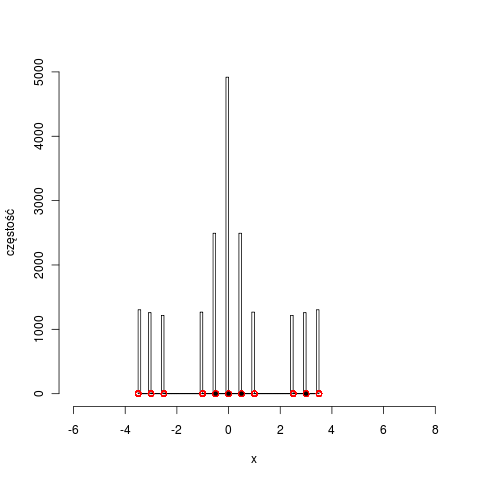
\includegraphics[width=.65\textwidth]{img/best}
\caption{Histogram mutantów dla DE/best/1} 
\label{fig:sym_best}
\end{figure}

\begin{figure}[H]
\centering
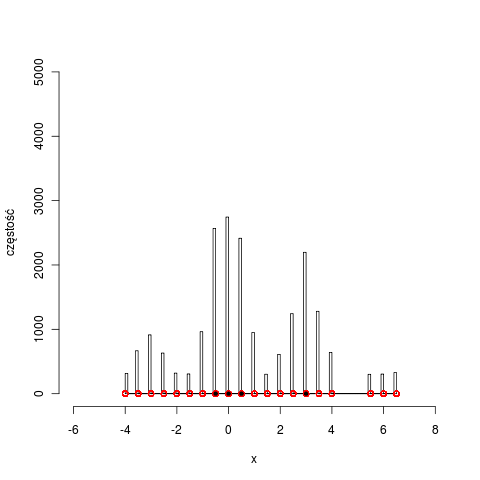
\includegraphics[width=.65\textwidth]{img/rand}
\caption{Histogram mutantów dla DE/rand/1} 
\label{fig:sym_rand}
\end{figure}


Wektor różnicowy dla DE/rand/1 oraz DE/best/1 ma postać $w = \sum\limits_{j=1}^k (P_{i_{2j}} - P_{i_{2j+1}})$. 
Rozkład wartości wektora $w$ jest symetryczny względem 0 i dąży do rozkładu Gaussa, gdy $k$ dąży do 
nieskończoności.

W przypadku DE/best/1 w selekcji wybierany był zawsze jeden ustalony punkt (najlepszy), 
a więc histogram (empiryczny rozkład) mutantów był symetryczny względem tego punktu.

Natomiast w przypadku DE/rand/1
w selekcji wybierany był punkt losowy. To sprawia, że wektory $w$ są dodawane
przeważnie do osobników o współrzędnej $x$ bliskiej 0 (są 3 takie punkty).
Z tego powodu histogram mutantów nie posiada osi symetrii i~zupełnie rożni się od tego uzyskanego dla DE/best/1.

\subsection{Wpływ liczby par wektów różnicowych $k$ na rozkład mutantów}

Mutanty, które sięgają
na tyle daleko, że umożliwiają wyjście z lokalnego optimum, są bardzo cenne. 
Ciągłe próbkowanie okolicznych, już zbadanych obszarów, na ogół nie przynosi korzyści.
W tym podrozdziale rozważana jest przestrzeń dwuwymiarowa.
Populacja początkowa przedstawiona na rysunku \ref{fig:10k_start} zawierała 20 punktów, 
przy czym 18 z nich leżało wokół osi $y = 0$. 
Jedynie 2 punkty wprowadzały większą różnorodność 
w wymiarze $y$: jeden o $y = 2.5$ oraz jeden o~$y = -2.5$. 

\begin{figure}[H]
\centering
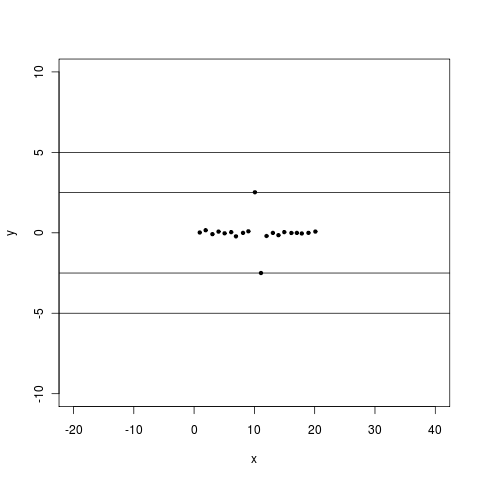
\includegraphics[width=.5\textwidth]{img/pop} 
\caption{20 punktów populacji początkowej} 
\label{fig:10k_start}
\end{figure}

Rysunek \ref{fig:10k_rand1} przedstawia 40 tysięcy mutantów wygerowanych zgodnie ze schematem DE/rand/1.
Rysunek \ref{fig:10k_rand6} przedstawia 40 tysięcy mutantów wygerowanych zgodnie ze schematem DE/rand/6.
Współczynnik skalujący $F$ dla 
DE/rand/1 wynosił 1, dla DE/rand/6 (zgodnie z tabelą \ref{table:wspolczynniki}) $\frac{1}{\sqrt{6}}$.

\begin{figure}[H]
\centering
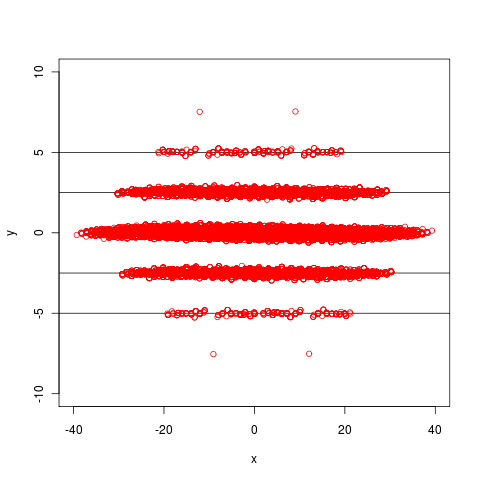
\includegraphics[width=.65\textwidth]{img/rand1}
\caption{40 tysięcy mutantów dla DE/rand/1} 
\label{fig:10k_rand1}
\end{figure}

\begin{figure}[H]
\centering
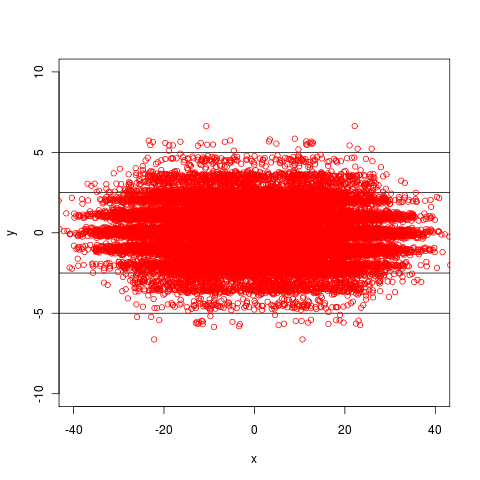
\includegraphics[width=.65\textwidth]{img/rand6}
\caption{40 tysięcy mutantów dla DE/rand/6} 
\label{fig:10k_rand6}
\end{figure}

Rozkład mutantów dla $k = 1$ nie przypomina rozkładu normalnego, 
natomiast dla $k = 6$ już upodabnia się do niego.

Liczba mutantów, dla których $|y| > 5$, 
znacznie się różniła w przypadku obu porównywanych schematów mutacji. 
Dla DE/rand/1 było to 352 mutantów,
natomiast dla DE/rand/6 jedynie 64. 

Ponadto, podczas mutacji DE/rand/1 pojawiły się 2 bardzo oddalone punkty o~$y > 7.5$. 
Żeby tak się zdarzyło, najpierw wylosowany musi zostać osobnik $P_{i_1}$ o~$y=2.5$.
Prawdopodobieństwo takiego zdarzenia wynosi $\frac{1}{20}$.
Następnie musi zostać wylosowany wektor różnicowy o~długości 5. Tylko jedna para punktów 
dawała taki wektor --
pierwszy punkt o $y = 2.5$, drugi punkt o $y = -2.5$. 
Prawdopodobieństwo wylosowania takiej pary wynosiło $\frac{1}{400}$. 
Zatem łączne prawdopodobieństwo powstania mutanta o~
$y~=~7.5$ dla DE/rand/1 wynosiło $\frac{1}{8000}$. 

Dla DE/rand/6 prawdopodobieństwo powstania mutanta o $y > 7.5$ jest mniejsze.
W celu oszacowania, przyjęto dla uproszczenia, że rozkład prawdopodobieństwa mutantów dla
DE/rand/6 jest wystarczająco zbliżony do DE/rand/$\infty$.
Zgodnie z opisem w rozdziale \ref{sub:de_rand_inf}, na początku wylosowany musi zostać osobnik 
$P_{i_1}$ o $y = 2.5$. Następnie musi zostać wygenerowana zmienna losowa 
$v_\infty$ o rozkładzie normalnym, której wartość w wymiarze $y$
przekroczy $5\sqrt{6} \approx 12.25$. Macierz kowariancji populacji początkowej  
$\C[P]$ wynosiła $\left[ \begin{array}{ c c }
  35.1798210 & -0.2902915 \\
  -0.2902915 &  0.6719438
\end{array} \right]$.
Wektor średnich~$m=\left[ \begin{array}{ c c } 10.463749675 & 0.004673205 \end{array} \right]$.
Prawdopodobieństwo wylosowania zmiennej o~$y > 5\sqrt{6}$ wynosi 
$1 - F(\infty, 5\sqrt{6}) \approx 0$.\footnote{Wartość ta jest tak mała,
że w reprezentacji liczb podwójnej precyzji użytych przy wywołaniu funkcji \texttt{pmvnorm} języka R
została uznana za 0.} $F$ to
dystrybuanta wielowymiarowego rozkładu $\mathcal{N}(m, \C[P])$.
Gdyby pierwszym wylosowanym punktem $P_{i_1}$ nie był ten o $y = 2.5$, tylko np. któryś 
z punktów leżących blisko osi $y = 0$, wówczas mutacja DE/rand/6 musiałaby wygenerować zmienną
o wartości $y$ większej niż $7.5\sqrt{6} \approx 18.37$. 
Prawdobieństwo takiego zdarzenia jest bliskie zeru.

\section{Algorytm DE/mid -- nowy wariant ewolucji różnicowej}

W poniższym podrozdziale przedstawiono nowy wariant ewolucji różnicowej wybierający w selekcji punkt środkowy populacji -- DE/mid.
Wybór punktu środkowego jest uzasadniony wynikiem pracy Zhanga oraz Sandersona, w której dowodzi się, że
środek populacji w DE ma zbieżność w sensie wartości oczekiwanej do wierzchołka paraboli optymalizowanej funkcji
\cite{zhang}. Punkt środkowy jest również wykorzystywany w bardzo efektywnym algorytmie CMA-ES
(ang. Covariance Matrix Adaptation Evolution Strategy) \cite{cmaes}.
Warianty tego algorytmu od lat zajmują najwyższe miejsca w konkursach typu BBOB \cite{setup} czy CEC \cite{cec}.

\subsection{Schemat algorytmu DE/mid/k}

W DE/mid/k mutant powstaje w następujący sposób:

\begin{equation} \label{eq:demid}
u_i^\text{mid} = m + F_\text{mid}\sum\limits_{j=1}^k (P_{i_{2j}} - P_{i_{2j+1}})
\end{equation}

gdzie $m$ to punkt środkowy populacji:
\begin{equation} \label{eq:midpoint}
m = \frac{1}{\mu}\sum\limits_{j=1}^n P_j
\end{equation}

$F_\text{mid}\in\mathbb{R_+}$ jest współczynnikiem skalującym dla DE/mid/k, analogicznym do $F$ 
w przypadku DE/rand/1 opisanego w rozdziale \ref{chap:de_rand}. 

\subsection{Analiza macierzy kowariancji generowanych mutantów}

Żeby macierz kowariancji populacji w DE/mid/k była taka sama jak w~DE/rand/1, 
macierz kowariancji mutanta $u_i^\text{mid}$ musi być taka sama jak macierz kowariancji mutanta $u_i$.
Można to osiągnąć tak dobierając $F_\text{mid}$, żeby było spełnione równanie:
\begin{equation} \label{eq:rownanie}
\C[u_i] = \C[u_i^\text{mid}]
\end{equation}

Rozwijając prawą stronę równania (\ref{eq:rownanie}):
\begin{equation}
\begin{align}
\label{eq:macierz_kow_mutanta_mid}
\C[u_i^\text{mid}] &\overset{\eqref{eq:demid}}{=} \C[m + F_\text{mid}\sum\limits_{j=1}^k (P_{i_{2j}} - P_{i_{2j+1}})] 
\overset{(\ref{eq:midpoint})}{=} \C[\frac{1}{\mu}\sum\limits_{j=1}^\mu P_j] + F_\text{mid}^2\C[\sum\limits_{j=1}^k (P_{i_{2j}} - P_{i_{2j+1}})] \\
&= \frac{1}{\mu^2}\mu\C[P] + F_\text{mid}^2\C[\sum\limits_{j=2}^{2k+1} P] = \C[P](2kF_\text{mid}^2 + \frac{1}{\mu})
\end{align}
\end{equation}

Przyrównując \eqref{eq:macierz_kow_mutanta} do \eqref{eq:macierz_kow_mutanta_mid}:
\begin{align*}
\C[P](2F^2 + 1) = \C[P](2kF_\text{mid}^2 + \frac{1}{\mu})
\end{align*}

Przy założeniu, że $\C[P] \neq \textbf{0}$:
\begin{align*}
2F^2 + 1 = 2kF_\text{mid}^2 + \frac{1}{\mu} \\
F_\text{mid}^2 = \frac{2F^2 + 1 - \frac{1}{\mu}}{2k}
\end{align*}

Obie strony są nieujemne, więc:
\begin{align} \label{eq:a}
F_\text{mid}\ = \sqrt{\frac{2F^2 + 1 - \frac{1}{\mu}}{2k}}
\end{align}

Zakładając dostatecznie duże wartości $\mu$, można przyjąć $\frac{1}{\mu} \approx 0$.
Wówczas \mbox{$F_\text{mid} \approx \sqrt{\frac{2F^2 + 1}{2k}}$}.
Przykładowo, współczynik skalujący dla DE/mid/1 równoważny DE/rand/1 przy $F = 0.9$ 
na mocy zależności \eqref{eq:a} wynosi $F_\text{mid} \approx 1.14$. \\

Przechodząc z $k$ do nieskończoności, równanie mutanta DE/mid/$\infty$ można zapisać
w następujący sposób:
\begin{align*}
u_i^{\infty^\text{mid}} = m + F_{\infty_\text{mid}} \cdot v_{\infty_\text{mid}}
\end{align*}

Gdzie współczynnik skalujący $F_{\infty_\text{mid}}$ jest równy $\sqrt{2F^2 + 1 - \frac{1}{\mu}}$, ponieważ:
\begin{align*}
\C[u_i^{\infty^\text{mid}}] &= \C[u_i] \\
\C[m + F_{\infty_\text{mid}} \cdot v_{\infty_\text{mid}}] &= \C[P](2F^2 + 1) \\
\frac{C[P]}{\mu} + F_{\infty_\text{mid}}^2 C[P] &= \C[P](2F^2 + 1) \\
F_{\infty_\text{mid}} &= \sqrt{2F^2 + 1 - \frac{1}{\mu}}
\end{align*}

\section{Współczynniki skalujące}

Tabela \ref{table:wspolczynniki} podsumowuje wyprowadzone współczynniki skalujące dla wszystkich
wariantów algorytmów analizowanych w tej pracy. Użycie tych współczynników gwarantuje, że macierz
kowariancji mutantów dla dowolnego wariantu ewolucji różnicowej będzie równa tej macierzy dla algorytmu
DE/rand/1 ze współczynikiem skalującym $F$.

Współczynniki skalujące dla DE/best są identyczne jak dla DE/mid, ponieważ w obu tych wariantach,
w iteracji dla bieżącej populacji, zawsze mutowany jest ten sam, ustalony punkt. 
W DE/rand punkt mutowany jest za każdym razem losowany, 
przez co jest bardziej zmienny (ma większą normę macierzy kowariancji).
Z tego powodu warianty DE/best oraz DE/mid potrzebują większych współczynników skalujących niż DE/rand.

\begin{table}[H]
\centering
\begin{tabular}{ l | c }
Algorytm         & Współczynnik skalujący równoważny $F$ z DE/rand/1 \\ \hline
DE/rand/k        & $\sqrt{\frac{2F^2}{2k}} = \frac{F}{\sqrt{k}}$ \\ 
DE/rand/$\infty$ & $\sqrt{2F^2} = \sqrt{2}F$ \\ \hline
DE/best/k        & $\sqrt{\frac{2F^2 + 1 - \frac{1}{\mu}}{2k}}$ \\
DE/best/$\infty$ & $\sqrt{2F^2 + 1 - \frac{1}{\mu}}$ \\ \hline
DE/mid/k         & $\sqrt{\frac{2F^2 + 1 - \frac{1}{\mu}}{2k}}$ \\
DE/mid/$\infty$  & $\sqrt{2F^2 + 1 - \frac{1}{\mu}}$ \\
\end{tabular}
\caption{Współczynniki skalujące dla algorytmów analizowanych w tej pracy gwarantujące równość macierzy kowariancji mutantów
dla DE/rand/1 ze współczynnikiem skalującym $F$}
\label{table:wspolczynniki}
\end{table}

\chapter{Metodyka testowania}
\label{chap:metodyka}

Twierdzenie No Free Lunch dla optymalizacji głosi, że nie istnieje najlepszy uniwersalny algorytm dla wszystkich zadań \cite{lunch}. 
Niezależnie od miary jakości algorytmu optymalizacyjnego, po uśrednieniu dla wszystkich zadań optymalizacyjnych, 
dowolne dwa różne algorytmy będą osiągały taką samą jakość wyników. Innymi słowy,
nie czyniąc żadnych założeń na temat natury optymalizowanej funkcji celu $f$, 
nigdy nie będziemy w stanie wykazać wyższości dowolnego algorytmu ewolucyjnego nad np. błądzeniem losowym. 
Zatem należy przyjąć pewne założenia na temat optymalizowanych funkcji, żeby móc wskazać algorytm najlepszy (dla danego zbioru funkcji).
W idealnym przypadku, funkcje testowe odpowiadałyby tym spotykanym w~rzeczywistych zadaniach optymalizacji.
Nie wiadomo jednak jakie rodziny funkcji występują najczęściej w realnych problemach.
Dlatego w tej pracy przyjęto zbiór 7 funkcji wybranych z~zestawu BBOB 2013 \cite{noiseless}, szczegółowo opisanych w poniższym rozdziale.

\section{Zestaw funkcji testowych BBOB 2013}
\label{sec:zestaw}

BBOB (ang. Black-Box Optimization Benchmarking) to nazwa warsztatów poświęconych testowaniu 
algorytmów optymalizacji \cite{setup}. 
Warsztaty te odbywały się w latach 2009, 2010, 2012 oraz 2013. 
Zmieniały się algorytmy startujące w konkursie, nie zmieniał
się sposób ich testowania. Podobnie funkcjonują warsztaty CEC (ang. Commission of the European Communities)
\cite{cec}.

W tej pracy wykorzystano funkcje z zestawu BBOB 2013. Wszystkie funkcje z tego zestawu
są zdefiniowane w całej przestrzeni $\mathbb{R}^D$, 
ale zbiór dopuszczalny został zawężony do $[-5; 5]^D$. 
Wszystkie poszukiwane minima leżą w tym obszarze.
Na rozwiązania spoza zbioru dopuszczalnego 
nakładana jest zewnętrzna funkcja kary zdefiniowana w \cite{setup} nastepująco: 

$$ f_\text{pen} : \mathbb{R}^D \rightarrow \mathbb{R}, 
\textbf{x} \mapsto \sum\limits_{i=1}^D \max\left(0, |x_i| - 5\right)^2 $$ 
\\
Zestaw BBOB 2013 składa się z 54 funkcji, które dzielą się na dwie zasadnicze klasy:

\begin{itemize}
 \item[$\bullet$] 24 funkcje bez szumów o numerach od 1 do 24 \cite{noiseless}. 
 \item[$\bullet$] 30 funkcji z szumami o numerach od 101 do 130 \cite{noisy}.
\end{itemize} 

Funkcje bez szumów zwracają dokładną wartość funkcji celu w punkcie $x$. Funkcje z szumami wartość tą dodatkowo modyfikują używając 
losowego szumu. W tej pracy skoncentrowano się na funkcjach bez szumów. Można je podzielić ze względu
na ich właściwości:

\begin{itemize}
 \item[$\bullet$] Funkcje separowalne (numery od 1 do 5).
 \item[$\bullet$] Funkcje dobrze uwarunkowane numerycznie (od 6 do 9).
 \item[$\bullet$] Funkcje jednomodalne (z jednym ekstremum lokalnym), źle uwarunkowane numerycznie (od 10 do 14).
 \item[$\bullet$] Funkcje wielomodalne o regularnej strukturze (od 15 do 19).
 \item[$\bullet$] Funkcje wielomodalne o nieregularnej strukturze (od 20 do 24).
\end{itemize} 

Zgodnie z procedurą BBOB 2013 \cite{setup}, 
celem algorytmu optymalizacji jest wygenerowanie rozwiązania o wartości funkcji celu mniejszej bądź 
równej od $f_\text{opt} + 10^{-8}$, gdzie $f_\text{opt}$ to minimum optymalizowanej funkcji. 
W wielu przypadkach znalezienie takiego rozwiązania trwałoby zbyt długo.
Dlatego zastosowano kryterium stopu,
jakim jest ograniczenie na maksymalną liczbę wywołań funkcji oceny ($FEs$, ang. Function Evaluations), wynoszącą $10^5D$. 
Rozmiar populacji $\mu$ dla każdego algorytmu wynosił $10D$. 
Początkowa populacja była inicjalizowana zgodnie z rozkładem jednostajnym w zbiorze dopuszczalnym tzn.
w hipersześcianie $[-5; 5]^D$. Punkty, które w czasie optymalizacji wyjdą poza zbiór 
dopuszczalny, nie są naprawiane. Zewnętrzna funkcja kary
zapobiega znacznemu oddalaniu się punktów od interesującego obszaru.

Ze wzlędu na losowość procesu optymalizacji, na każdej funkcji algorytm jest uruchamiany 15 razy.
Z każdego uruchomienia zapisywany jest najlepszy wynik będący wartością funkcji dla najlepszego osobnika
pomniejszoną o $f_\text{opt}$.

Na funkcjach separowalnych, dobrze uwarunkowanych numerycznie lub jednomodalnych ewolucja różnicowa znajdowała rozwiązanie
bliskie optymalnemu na tyle często, że kłopotliwe było porównywanie jej wariantów. 
Różnice pomiędzy wariantami algorytmów udało się uchwycić przy użyciu trudniejszych funkcji.
Z tego powodu wybrano 7 funkcji 
wielomodalnych o numerach 15, 16, 19, 20, 21, 22, 24. Trzy z nich mają regularną strukturę (15, 16, 19), 
cztery nieregularną (20, 21, 22, 24). Wszystkie są niesymetryczne.
Poniżej przedstawiono je dokładniej.
Na trójwymiarowych wykresach wartości funkcji $f$ maleją ku górze, 
żeby minima globalne funkcji były dobrze widoczne.
Dlatego minimalizacja oznacza ,,wchodzenie pod górę''.

\subsection{Funkcja numer 15 -- Rastrigina}

Ekstrema w oryginalnej funkcji Rastrigina są rozmieszczone regularnie i symetryczne. Dzięki dwóm transformacjom $T^\beta_\text{asy}$ 
oraz $T_\text{osz}$ zaburzono symetrię oraz regularność. Właściwości funkcji numer 15: 
\begin{itemize}
 \item[$\bullet$] Około $10D$ minimów lokalnych.
 \item[$\bullet$] Globalnie duże zmiany wartości, lokalnie - małe.
 \item[$\bullet$] Separowalna liniowo.
\end{itemize} 

$$ f_{15}(\bold{x}) = 10 \left( D - \sum^D_{i=1}\cos(2 \pi z_i) \right) + \norm{\bold{z}}^2 + f_\text{opt} $$
$$ \bold{z} = \bold{R} \bold{\Lambda}^{10} \bold{Q} T^{0.2}_\text{asy}(T_\text{osz}(\bold{R}(\bold{x} - \bold{x}^\text{opt}))) $$ 

$\bold{Q}$ i $\bold{R}$ to ortogonalne macierze obrotu.
$\bold{\Lambda}^\alpha$ to $D$-wymiarowa macierz diagonalna, w której $i$-ty element na przekątnej jest równy 
$\alpha^{\frac{1}{2}\frac{i-1}{D-1}}$ dla $i = 1, \dots, D$.

\begin{figure}[H]
\centering
\mbox{
\includegraphics[width=.45\textwidth]{img/15.png} \quad
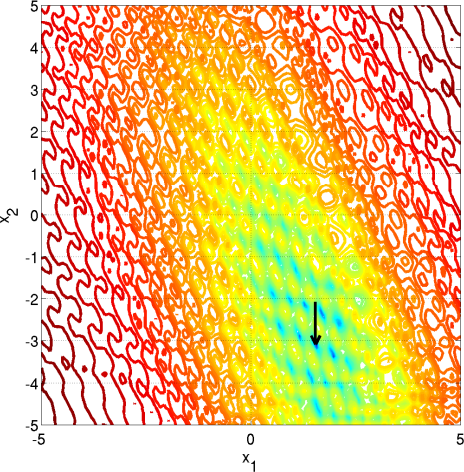
\includegraphics[width=.45\textwidth]{img/15a.png} 
}
\caption{Dwuwymiarowa funkcja Rastrigina, strzałka wskazuje minimum \cite{noiseless}}
\end{figure}

\subsection{Funkcja numer 16 -- Weierstrassa}

Funkcja 16 jest obrócona w stosunku do oryginalnej funkcji Weierstrassa -- pierwszego opublikowanego przykładu
rzeczywistej funkcji ciągłej, nieróżniczkowalnej w żadnym punkcie \cite{szarek}.
Posiada powtarzalny, ale bardzo ,,wyboisty'' przebieg oraz więcej niż jedno optimum globalne. Właściwości:
\begin{itemize}
 \item[$\bullet$] Globalnie regularna, lokalnie nieregularna.
 \item[$\bullet$] Brak unikalnego optimum globalnego.
\end{itemize} 

$$ f_{16}(\bold{x}) = 10 \left( \frac{1}{D} \sum^D_{i=1} \sum^{11}_{k=0} 1 / 2^k \cos(2 \pi 3^k(z_i + 1/2)) - f_0 \right)^3 + \frac{10}{D} f_\text{pen}(\bold{x}) + f_\text{opt} $$
$$ \bold{z} = \bold{R} \bold{\Lambda}^{1/100} \bold{Q} T_\text{osz}(\bold{R}(\bold{x} - \bold{x}^\text{opt})) $$
$$ f_0 = \sum^{11}_{k=0} 1/2^k \cos(2 \pi 3^k 1/2) $$

\begin{figure}[H]
\centering
\mbox{
\includegraphics[width=.45\textwidth]{img/16.png} \quad
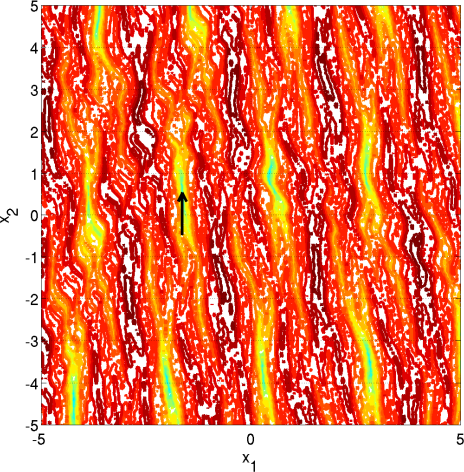
\includegraphics[width=.45\textwidth]{img/16a.png} 
}
\caption{Dwuwymiarowa funkcja Weierstrassa, strzałka wskazuje minimum \cite{noiseless}}
\end{figure}

\subsection{Funkcja numer 19 -- Griewanka-Rosenbrocka}

Funkcja 19 to złożenie funkcji Griewanka oraz Rosenbrocka, o ogromnej liczbie ekstremów lokalnych.
$$ f_{19}(\bold{x}) = \frac{10}{D - 1} \sum^{D-1}_{i=1}\left(\frac{s_i}{4000} - \cos(s_i)\right) + 10 + f_\text{opt} $$
$$ \bold{z} = \max\left(1, \frac{\sqrt{d}}{8}\right) \bold{Rx} + 0.5 $$
$$ \bigwedge_{i \in 1, \dots, D} s_i = 100(z^2_i - z_{i+1})^2 + (z_i - 1)^2 $$
$$ \bold{z}^\text{opt} = \bold{1} $$

\begin{figure}[H]
\centering
\mbox{
\includegraphics[width=.45\textwidth]{img/19.png} \quad
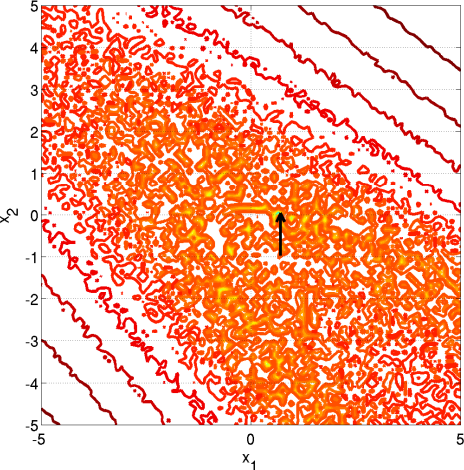
\includegraphics[width=.45\textwidth]{img/19a.png} 
}
\caption{Dwuwymiarowa funkcja numer 19, strzałka wskazuje minimum \cite{noiseless}}
\end{figure}

\subsection{Funkcja numer 20 -- Schwefela}

$\bold{1}^+_-$ oznacza wektor długości $D$ zawierający 1 oraz -1 losowane z równym prawdopodobieństwem.
W funkcji Schwefela najlepsze $2^D$ minimów lokalnych jest położonych stosunkowo blisko narożników atrakcyjnej hiperpłaszczyzny. Właściwości:
\begin{itemize}
 \item[$\bullet$] Częściowo separowalna.
 \item[$\bullet$] Charakterystyczna, obrócona struktura.
 \item[$\bullet$] Atrakcyjne obszary przeszukiwań znajdują się w narożnikach hiperpłaszczyzny.
\end{itemize} 

$$ f_{20}(\bold{x}) = -\frac{1}{D} \sum^D_{i=1} z_i \sin\left(\sqrt{|z_i|}\right) + 4.189828872724339 + 100 f_\text{pen}\left(\frac{\bold{z}}{100}\right) + f_\text{opt} $$
$$ \hat{\bold{x}} = 2 \cdot \bold{1}^+_- \otimes \bold{x} $$
$$ \bigwedge_{i \in 1, \dots, D} \hat{z}_1 = \hat{x}_1, \hat{z}_{i+1} = \hat{x}_{i+1} + 0.25(\hat{x}_i - x_i^\text{opt}) $$ 
$$ \bold{x}^\text{opt} = \frac{4.2096874633}{2} \bold{1}^+_- $$

\begin{figure}[H]
\centering
\mbox{
\includegraphics[width=.45\textwidth]{img/20.png} \quad
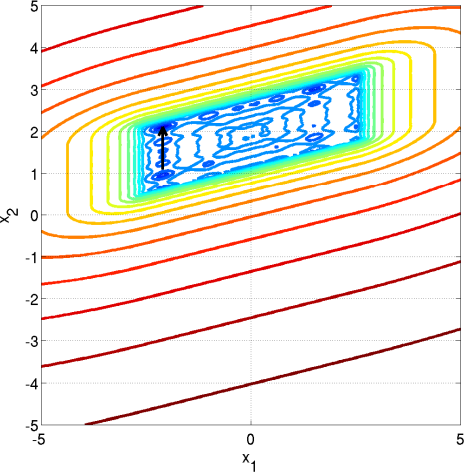
\includegraphics[width=.45\textwidth]{img/20a.png} 
}
\caption{Dwuwymiarowa funkcja Schwefela, strzałka wskazuje minimum \cite{noiseless}}
\end{figure}

\subsection{Funkcja numer 21 -- górki gaussowskie Gallaghera 101-me}

Funkcja posiada 101 ekstremów lokalnych, których położenie oraz wielkość są losowe i~niezależne od siebie.
Analizowanie wyników na tej funkcji pomaga odpowiedź na pytanie, czy przeszukiwanie jest efektywne, 
gdy funkcja celu nie ma żadnej globalnej struktury.
$$ f_{21}(\bold{x}) = T_\text{osz}\left(10-\max_{i=1}^{101}w_i\exp\left(-\frac{1}{2D}(\bold{x}-\bold{y}_i)^T\bold{R}^T\bold{C}_i\bold{R}(\bold{x}-\bold{y}_i)\right)\right)^2 + f_\text{pen}(\bold{x}) + f_\text{opt} $$
\[
w_i =
\begin{cases} 
1.1 + 8 \cdot \frac{i-2}{99} & \mbox{dla } i = 2, \dots, 101 \\ 
10 & \mbox{dla } i = 1
\end{cases}
\] 
$\bold{C}_i$ jest zdefiniowane w \cite{noiseless}. 

\begin{figure}[H]
\centering
\mbox{
\includegraphics[width=.45\textwidth]{img/21.png} \quad
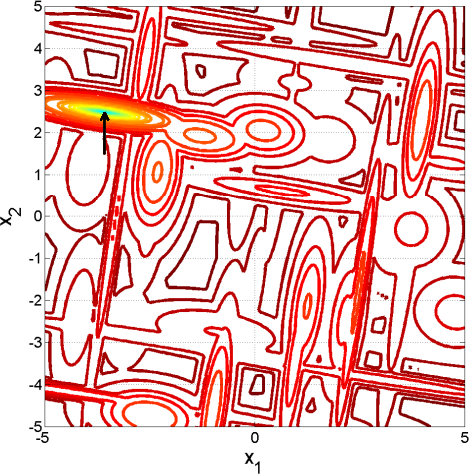
\includegraphics[width=.45\textwidth]{img/21a.png} 
}
\caption{Dwuwymiarowa funkcja numer 21, strzałka wskazuje minimum \cite{noiseless}}
\end{figure}

\subsection{Funkcja numer 22 -- górki gaussowskie Gallaghera 21-hi}

Funkcja posiada 21 ekstremów lokalnych, których położenie oraz wielkość są losowe i~niezależne od siebie.
Analizowanie wyników na tej funkcji pomaga odpowiedź na pytanie, 
jak wysoki wskaźnik uwarunkowania numerycznego wpływa na efektywność przeszukiwania,
w~porównaniu do funkcji 21.
$$ f_{22}(\bold{x}) = T_\text{osz}\left(10-\max_{i=1}^{21}w_i\exp\left(-\frac{1}{2D}(\bold{x}-\bold{y}_i)^T\bold{R}^T\bold{C}_i\bold{R}(\bold{x}-\bold{y}_i)\right)\right)^2 + f_\text{pen}(\bold{x}) + f_\text{opt} $$
\[
w_i =
\begin{cases} 
1.1 + 8 \cdot \frac{i-2}{19} & \mbox{dla } i = 2, \dots, 21 \\ 
10 & \mbox{dla } i = 1
\end{cases}
\] 
$\bold{C}_i$ zostało zdefiniowane w \cite{noiseless}. 

\begin{figure}[H]
\centering
\mbox{
\includegraphics[width=.45\textwidth]{img/22.png} \quad
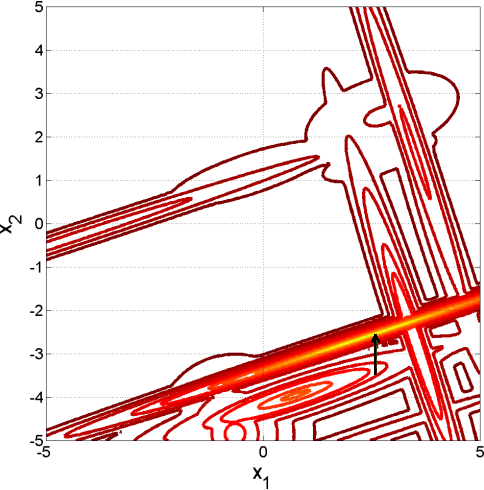
\includegraphics[width=.45\textwidth]{img/22a.png} 
}
\caption{Dwuwymiarowa funkcja numer 22, strzałka wskazuje minimum \cite{noiseless}}
\end{figure}

\subsection{Funkcja numer 24 -- Lunačka}

Funkcja Lunačka jest również nazywana podwójnym Rastriginem (bi-Rastrigin). Funkcja ta ma dużą liczbę ekstremów lokalnych. 
Na jej dwuwymiarowym wykresie można zauważyć dwa charekterystyczne zbiory przyciągania 
minimum lokalnego -- ,,górki''. 
Żeby znaleźć optimum, algorytm optymalizacji musi najpierw poprawnie wybrać ,,górkę'',
a następnie dokładnie przeszukać wielomodalny obszar wewnątrz jej. Funkcja została skonstruowana w taki sposób, aby zmylić
niektóre algorytmy ewolucyjne z dużym rozmiarem populacji. Obszar przyciągania zawierający zwodnicze
minimum lokalne stanowi około 70\% całej przestrzeni przeszukiwań.
Analiza wyników na tej funkcji pomaga odpowiedzieć na pytanie,
czy przeszukiwanie może mieć charakter lokalny w~skali globalnej 
oraz charakter globalny w skali lokalnej.
$$ f_{24}(\bold{x}) = \min \left( \sum^D_{i=1}(\hat{x}_i - \mu_0)^2, dD + s \sum^D_{i=1}(\hat{x}_i - \mu_1)^2 \right) + 10 \left( D - \sum^D_{i=1} \cos(2 \pi z_i) \right) + 10^4 f_\text{pen}(\bold{x}) $$
$$ \hat{\bold{x}} = 2 \text{ sign}(\bold{x}^{\text{opt}}) \otimes \bold{x}, \bold{x}^{\text{opt}} = \mu_0 \bold{1}_-^+ $$
$$ \bold{z} = \bold{Q}\Lambda^{100}\bold{R}(\hat{\bold{x}} - \mu_0\bold{1}) $$
$$ \mu_0 = 2.5, \mu_1 = -\sqrt{\frac{\mu_0^2-d}{s}}, s = 1 - \frac{1}{2\sqrt{D+20}-8.2}, d=1 $$

\begin{figure}[H]
\centering
\mbox{
\includegraphics[width=.45\textwidth]{img/24.png} \quad
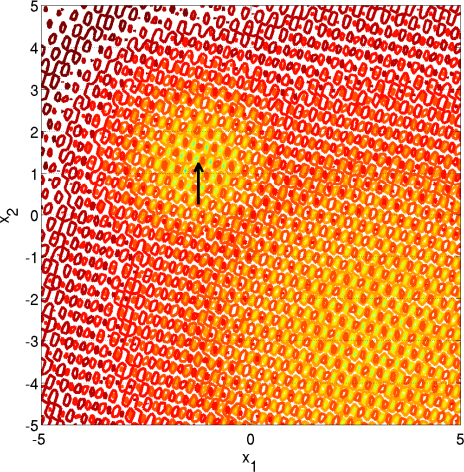
\includegraphics[width=.45\textwidth]{img/24a.png} 
}
\caption{Dwuwymiarowa funkcja Lunačka, strzałka wskazuje minimum \cite{noiseless}}
\end{figure}

\section{Porównywanie wyników}

Duża liczba wariantów algorytmów wymaga systematycznego i wiarygodnego sposobu porównywania
i prezentacji wyników. Testy istotności statystycznej pozwalają w~szybki sposób rozstrzygnąć, czy 
wyniki osiągane przez dwa algorytmy są od siebie różne w statystycznie istotny sposób.
Statystycznie istotny, to znaczy, czy obserwowane różnice wyników nie są jedynice wynikiem losowości związanej
z niedeterministycznym charakterem porównywanych algorytmów.
Dystrybuanty empiryczne
pozwalają zorientować się na ile wyniki algorytmów różnią się od siebie. Procent osobników, które
znalazły się poza przestrzenią przeszukiwań, pozwala ocenić, czy algorytm dotarł do krawędzi
zbioru dopuszczalnego, czy pozostawał cały czas w jego wnętrzu.

\subsection{Testy istotności statystycznej}
\label{sec:testy_istotnosci}

W tej pracy jako podstawowy sposób porównywania wyników został wykorzystany test 
Wilcoxona dla par obserwacji. Zaproponowany pierwotnie jako test przesunięcia dla dwóch równolicznych 
próbek przez Franka Wilcoxona w 1945, uogólniony następnie przez Manna i Whitneya w 1947
dla przypadku różnolicznych próbek \cite{mann}. Test Wilcoxona to nieparametryczna alternatywa dla testu t-Studenta w 
przypadku dwóch równolicznych próbek. Test t-Studenta sprawdza hipotezę zerową o równości
średnich arytmetycznych w odpowiadających im populacjach, natomiast test Wilcoxona
weryfikuje równość median. Średnia jest wrażliwa na wartości odstające,
natomiast mediana nie. Ponadto, test t-Studenta jest parametryczny, to znaczy zakłada pewien rozkład
wartości z badanej próby. Test Wilcoxona jest nieparametryczny, to znaczy,
nie zakłada postaci rozkładu badanych wartości. Dlatego został wybrany.

W teście Wilcoxona porównywane jest $n$ par obserwacji, pochodzących z dwóch zbiorów. 
Pierwszy zbiór odpowiada algorytmowi A i zawiera
liczby $x_1, x_2, \dots, x_{n}$. 
Drugi zbiór odpowiada algorytmowi B i zawiera 
liczby $y_1, y_2, \dots, y_{n}$. 
Liczby w zbiorach oznaczają różnice wartości funkcji celu najlepszego punktu oraz minimum globalnego
optymalizowanej funkcji. 
W tej pracy $n=15$,
ponieważ liczba niezależnych uruchomień algorytmu wynosiła 15.
Zostały spełnione wszystkie założenia dla testu Wilcoxona:

\begin{enumerate}
 \item Wartości $x_i$ i $y_i$ są parowane w sposób losowo niezależny od siebie. 
 \item Wartości $x_i$ i $y_i$ pochodzą z populacji o rozkładzie ciągłym.
 \item Wartości $x_i$ i $y_i$ można porównywać ze sobą, jednoznacznie stwierdzając,
która jest większa, mniejsza,
bądź równa.
\end{enumerate}

Testowana hipoteza zerowa $H_0$ brzmi: ,,różnica pomiędzy medianami rozkładów generujących zbiory A i B wynosi zero''.
Hipoteza alternatywna $H_1$ brzmi: ,,różnica pomiędzy medianami rozkładów generujących zbiory A i B jest różna od zera''.
Test Wilcoxona przebiega następująco:

\begin{enumerate}
 \item Obliczenie różnic $d_i = y_i - x_i$.
 \item Usunięcie par, dla których $d_i = 0$. $N \leq n$ oznacza liczbę pozostałych par.
 \item Posortowanie rosnąco wartości bezwględnych różnic $|d_i|$.
 \item Rangowanie posortowanego zbioru rangami $R_i$, poczynając od rangi równej 1. 
 \item Obliczenie statystyki $W = |\sum\limits_{i=1}^{N} \sgn(d_i)R_i|$.
 \item Rozkład $W$ zbiega do rozkładu normalnego wraz ze wzrostem $N$. Obliczane jest
 $p = \frac{W - 0.5}{\sigma_W}$, gdzie $\sigma_W = \sqrt{\frac{N(N+1)(2N+1)}{6}}.$ 
 \item Jeśli $z > z_\text{critical}$, hipoteza $H_0$ jest odrzucana, w przeciwnym przypadku -- przyjmowana. 
Wartości $z_\text{critical}$ zależą od przyjętego poziomu ufności. 
W tej pracy poziom ufności wynosił $0.05$, co odpowiada $z_\text{critical}=1.96$ \cite{lowry}.  
\end{enumerate}

Jeśli test nie pozwalał na odrzucenie hipotezy zerowej, uznawano, że wyniki porównywanych algorytmów
nie są istotnie różne od siebie. 
Jeśli test odrzucał hipotezę zerową, uznawano, że algorytmy A i B dają różne wyniki.
Wówczas porówywane były mediany obu zbiorów. Algorytm, którego mediana wyników była niższa,
uznawany był za lepszy.

\subsection{Dystrybuanty empiryczne}
\label{sec:dystrybuanty}

W celu porównania wyników osiąganych przez algorytmy, 
wykreślono dystrybuanty empiryczne najlepszych wyników z każdego uruchomienia 
dla wszystkich algorytmów na jednej funkcji. Oś $x$ wykresu
odpowiada wartościom najlepszych wyników osiąganych przez algorytmy, 
tzn. różnicom wartości funkcji celu najlepszego
punktu wyznaczonego w pojedynczym uruchomieniu 
oraz minimum globalnego optymalizowanej funkcji. Oś $y$ odpowiada natomiast 
estymowanemu prawdopodobieństwu, z jakim algorytm osiąga dany wynik. 
Dystrybuanty empiryczne pozwalają również
określić, jak bliskie minimum było najlepsze znalezione przez algorytm rozwiązanie.

\subsection{Procent osobników poza zbiorem dopuszczalnym}

W każdym uruchomieniu zliczana była liczba osobników, których jakakolwiek współrzędna wykraczała poza
zbiór dopuszczalny zdefiniowany jako $[-5; 5]^D$. Następnie obliczany był stosunek liczby 
osobników spoza zbioru dopuszczalnego do liczby wszystkich wygenerowanych osobników. Jeśli algorytm
nie znajdował minimum, wówczas liczba wszystkich generowanych osobników była równa maksymalnej
liczbie obliczeń wartości funkcji celu $FEs = 10^5D$. 
Dla jednego algorytmu i jednej funkcji, procent osobników
poza zbiorem dopuszczalnym uśredniano z 15 niezależnych uruchomień.

\chapter{Wyniki eksperymentów}

W tym rozdziale przedstawiono najważniejsze wyniki eksperymentów opatrzone komentarzem.
Wszystkie wykresy oraz dane tabelaryczne znajdują się w dodatku B.

\section{Parametry eksperymentów}

Dla funkcji o małej liczbie wymiarów trudno dostrzec różnicę pomiędzy algorytmami. 
Im wyższy wymiar przestrzeni przeszukiwań,
tym trudniejszy problem i dłuższy czas obliczeń, ale różnice pomiędzy efektywnością
badanych algorytmów stają się bardziej widoczne.
 Dlatego liczba wymiarów $D$ w testach wynosiła 10, 20, 40 oraz 80. 

Współczynnik skalujący algorytmu DE/rand/1 wynosił $F = 0.9$. 
Dla pozostałych algorytmów współczynnik skalujący był obliczany zgodnie z tabelą
\ref{table:wspolczynniki}.
W każdym z~algorytmów zostało wykorzystane krzyżowanie dwumianowe (opisane w rozdziale
\ref{sec:krzyzowanie}) ze
współczynnikiem krzyżowania $CR = 0.9$ \cite{ronkkonen}.

\section{Implementacja}

Zestaw BBOB 2013 dostarcza implementację wszystkich funkcji testowych w języku C. Funkcje te obliczane
są miliardy razy podczas eksperymentów, dlatego ważne jest, żeby wykonywały się jak najszybciej.
Procedura testująca oraz badane algorytmy zostały zaimplementowane w 
Javie. Procedura testująca wywołuje funkcje napisane w~języku~C~dzięki Java Native Interface (JNI).
Do automatyzacji testów oraz przetwarzania wyników zostały napisane skrypty w sh 
(języku powłoki Bourne'a) oraz języku~R. Do przeprowadzenia testów istotności statystycznej Wilcoxona 
użyto funkcji \texttt{wilcox.test} z pakietu \texttt{stats} języka R. Dystrybuanty empiryczne
zostały obliczone dzięki funkcji \texttt{ecdf} (ang. empirical cumulative distribution function),
pochodzącej z tego samego pakietu.

Poprawność implementacji algorytmów w Javie została zweryfikowana dzięki testom macierzy kowariancji
populacji. Zbadano wartości macierzy po pierwszej mutacji, uśrednione z~10000 niezależnych uruchomień. 
Średnie wartości macierzy kowariancji były bardzo zbliżone dla wszystkich badanych algorytmów, 
zgodnie z założeniami teoretycznymi poczynionymi w rozdziale
\ref{chap:de_mid}. Uśrednioną macierz kowariancji populacji przedstawia tabela 
\ref{table:cov_matrix}. 

\begin{table}[H]
\centering
\begin{tabular}{ c c c c c c c c c c }
21.36 & 0.02 & 0.01 & -0.04 & 0.06 & -0.01 & -0.03 & -0.02 & -0.01 & 0.03 \\
0.02 & 21.37 & 0.00 & 0.01 & -0.01 & 0.02 & 0.03 & 0.02 & 0.03 & 0.00 \\
0.01 & 0.00 & 21.40 & -0.01 & -0.03 & -0.03 & -0.09 & 0.04 & 0.01 & -0.02 \\
-0.04 & 0.01 & -0.01 & 21.37 & 0.02 & 0.00 & 0.02 & 0.07 & 0.03 & -0.03 \\
0.06 & -0.01 & -0.03 & 0.02 & 21.43 & -0.00 & 0.02 & 0.01 & -0.01 & 0.01 \\
-0.01 & 0.02 & -0.03 & 0.00 & -0.00 & 21.41 & -0.00 & -0.01 & 0.02 & -0.01 \\
-0.03 & 0.03 & -0.09 & 0.02 & 0.02 & -0.00 & 21.38 & 0.04 & 0.05 & -0.01 \\
-0.02 & 0.02 & 0.04 & 0.07 & 0.01 & -0.01 & 0.04 & 21.40 & -0.05 & 0.04 \\
-0.01 & 0.03 & 0.01 & 0.03 & -0.01 &  0.02 & 0.05 & -0.05 & 21.39 & 0.02 \\
0.03 & 0.00 & -0.02 & -0.03 & 0.01 & -0.01 & -0.01 &  0.04 & 0.02 & 21.37 \\
\end{tabular}
\caption{Uśredniona macierz kowariancji dla 10-wymiarowej funkcji numer 15 i~algorytmu DE/rand/1.}
\label{table:cov_matrix}
\end{table}

Wszystkie funkcje użyte do testów są nieseparowalne liniowo.
Dlatego wartości macierzy kowariancji populacji poza główną przekątną są bliskie 0. Oznacza to,
iż korelacja liniowa Pearsona pomiędzy wartościami różnych cech praktycznie nie występuje, wymiary
są niezależne od siebie. Z kolei wartość bliska 21.4 powtarzająca się na głównej przekątnej 
oznacza taką samą wariancję wartości w każdym z wymiarów, tzn. dla każdej cechy osobnika.
Przedstawiona macierz kowariancji jest praktycznie taka sama dla wszystkich algorytmów, 
dzięki odpowiednim współczynnikom skalującym
$F$ wyprowadzonym w rozdziale \ref{chap:de_mid} oraz identycznym populacjom początkowym. 
Dzięki niemal identycznej macierzy kowariancji algorytmy
mają taki sam zasięg mutacji i wyniki przez nie zwracane zależą tylko od badanego sposobu selekcji.
Wartość bliską 21.4 można uzasadnić dzięki wyprowadzonej zależności \eqref{eq:macierz_kow_mutanta},
wiążącej macierz kowariancji mutanta $\C[u_i]$
z macierzą kowariancji początkowej populacji $\C[P]$. Populacja początkowa była losowana zgodnie z 
rozkładem jednostajnym na przedziale $[-5;5]^{10}$, zatem na głównej przekątnej $\C[P]$
znajduje się liczba $\frac{10^2}{12} \approx 8.3$, zgodnie ze wzorem na wariancję rozkładu jednostajnego 
$\frac{(b - a)^2}{12}$. $F$ było równe 0.9, zatem 
$\C[u_i] = \C[P](2 \cdot 0.9^2 + 1) = \C[P] \cdot 2.62 \approx \bold{\Lambda_{10}} \cdot 8.3 \cdot 2.62 \approx \bold{\Lambda_{10}} \cdot 21.7$, gdzie $\bold{\Lambda_{10}}$
to 10-wymiarowa macierz diagonalna. 

\section{Wnioski}

W notacji stosowanej w tabelach brak statystycznej różnicy oznaczono znakiem ,,$\cdotp$''.
Jeśli test istotności (opisany w rozdziale \ref{sec:testy_istotnosci})
odrzucał hipotezę zerową, uznawano, że algorytmy A i B dają różne wyniki.
Wówczas porówywane były mediany obu zbiorów. Algorytm, którego mediana wyników była niższa,
uznawany był za lepszy i oznaczany znakiem ,,+''. Algorytm istotnie gorszy był oznaczany znakiem ,,--''.

W tabeli \ref{table:demid80} przedstawiono porównanie wariantu DE/mid/1 do pozostałych, w~80~wymiarach.
DE/mid/1 dawał lepsze rezultaty niemal dla wszystkich przypadków, jedynie na funkcji 16 zremisował z DE/rand/1
oraz uległ DE/best/1.

\begin{table}[H]
\centering
\begin{tabular}{ | l | c | c | c | c | c | c | c | }
\hline		 & \multicolumn{7}{c |}{Numer funkcji testowej}  \\  \hline
Algorytm         &15& 16& 19& 20& 21& 22& 24 \\ \hline
DE/rand/1	 & + & $\cdot$ & + & + & + & + & + \\
DE/rand/2	 & + & + & + & + & + & + & + \\
DE/rand/6	 & + & + & + & + & + & + & + \\
DE/rand/$\infty$	 & + & + & + & + & + & + & + \\
DE/best/1	 & + & -- & + & + & + & + & + \\
DE/best/2	 & + & + & + & + & + & + & + \\
DE/best/6	 & + & + & + & + & + & + & + \\
DE/best/$\infty$	 & + & + & + & + & + & + & + \\
DE/mid/2	 & + & + & + & + & + & + & + \\
DE/mid/6	 & + & + & + & + & + & + & + \\
DE/mid/$\infty$	 & + & + & + & + & + & + & + \\ \hline
\end{tabular}
\caption{Porównanie DE/mid/1 do reszty wariantów DE w 80 wymiarach}
\label{table:demid80}
\end{table}

Istnieje jednak nieskończenie wiele funkcji dla których DE/mid/1 nie jest najlepszym wyborem, np. rodzina
funkcji podobnych do funkcji numer 16 -- Weierstrassa. Na takich funkcjach lepiej sprawuje się 
DE/best/1. 

Przetestowano również wariant algorytmu, w którym dla każdej populacji obliczano punkt środkowy,
a następnie wywoływano dla niego funkcję oceny, w nadziei znalezienia najlepszego rozwiązania.
Punkt ten nie był brany jako punkt do populacji. Wyniki otrzymywane po takiej modyfikacji nie różniły
się w~sposób statystycznie istotny w~porównaniu z~oryginalnym podejściem.

Biorąc pod uwagę najwyższy zbadany wymiar i wszystkie 7 funkcji testowych,
końcowy ranking efektywności algorytmów, opracowany na podstawie porównań testów Wilcoxona
dla wyników symulacji na 7 wybranych funkcjach, przedstawia się 
nastepująco:

\begin{enumerate}
 \item DE/mid/1
 \item DE/rand/1
 \item DE/best/1
 \item DE/mid/2
 \item DE/rand/2
 \item DE/best/2
 \item DE/mid/6, DE/mid/$\infty$, DE/rand/6, DE/rand/$\infty$, DE/best/6, DE/best/$\infty$
\end{enumerate}

\subsection{Wpływ liczby wymiarów na jakość rozwiązań}

Wraz ze wzrostem liczby wymiarów, algorytm DE/mid/1 sprawuje się coraz lepiej w porównaniu do
pozostałych wariantów.
W~80~wymiarach jednoznacznie wygrywa ze wszystkimi pozostałymi algorytmami na 6~z~7~funkcji testowych.
W~40~wymiarach prowadzenie DE/mid/1 wygląda podobnie. Jedynie różnica w~stosunku do DE/rand/1
jest mniejsza, z którym to DE/mid/1 wygrywa na 3 funkcjach, remisuje również na 3, a~na 1~przegrywa.
W~20~wymiarach zajmuje drugie miejsce, ustępując DE/rand/1.
W~10~wymiarach było najwięcej remisów,
DE/mid/1 był zawsze najlepszy na funkcjach numer 15, 19 oraz 24.

\begin{table}[H]
\centering
\begin{tabular}{ | l | c | c | c | c | c | c | c | }
\hline		 & \multicolumn{7}{c |}{Numer funkcji testowej}  \\  \hline
Algorytm         &15& 16& 19& 20& 21& 22& 24 \\ \hline
DE/rand/1	 & + & $\cdot$ & + & -- & $\cdot$ & $\cdot$ & + \\
DE/rand/2	 & + & + & + & + & + & + & + \\
DE/rand/6	 & + & + & + & + & + & + & + \\
DE/rand/$\infty$	 & + & + & + & + & + & + & + \\
DE/best/1	 & + & -- & + & + & + & + & + \\
DE/best/2	 & + & + & + & + & + & + & + \\
DE/best/6	 & + & + & + & + & + & + & + \\
DE/best/$\infty$	 & + & + & + & + & + & + & + \\
DE/mid/2	 & + & + & + & + & + & + & + \\
DE/mid/6	 & + & + & + & + & + & + & + \\
DE/mid/$\infty$	 & + & + & + & + & + & + & + \\ \hline
\end{tabular}
\caption{Porównanie DE/mid/1 do reszty wariantów DE w 40 wymiarach}
\end{table}

\begin{table}[H]
\centering
\begin{tabular}{ | l | c | c | c | c | c | c | c | }
\hline		 & \multicolumn{7}{c |}{Numer funkcji testowej}  \\  \hline
Algorytm         &15& 16& 19& 20& 21& 22& 24 \\ \hline
DE/rand/1	 & $\cdot$ & -- & $\cdot$ & -- & $\cdot$ & $\cdot$ & -- \\
DE/rand/2	 & + & + & + & $\cdot$ & $\cdot$ & $\cdot$ & + \\
DE/rand/6	 & + & + & + & + & + & $\cdot$ & + \\
DE/rand/$\infty$	 & + & + & + & $\cdot$ & + & $\cdot$ & + \\ 
DE/best/1	 & + & -- & + & -- & + & + & + \\
DE/best/2	 & + & + & + & + & + & + & + \\
DE/best/6	 & + & + & + & + & + & + & + \\
DE/best/$\infty$	 & + & + & + & + & + & + & + \\
DE/mid/2	 & + & + & + & $\cdot$ & + & $\cdot$ & + \\
DE/mid/6	 & + & + & + & $\cdot$ & + & $\cdot$ & + \\
DE/mid/$\infty$	 & + & + & + & $\cdot$ & + & $\cdot$ & + \\ \hline
\end{tabular}
\caption{Porównanie DE/mid/1 do reszty wariantów DE w 20 wymiarach}
\end{table}

\begin{table}[H]
\centering
\begin{tabular}{ | l | c | c | c | c | c | c | c | }
\hline		 & \multicolumn{7}{c |}{Numer funkcji testowej}  \\  \hline
Algorytm         &15& 16& 19& 20& 21& 22& 24 \\ \hline
DE/rand/1	 & + & -- & + & -- & $\cdot$ & $\cdot$ & + \\
DE/rand/2	 & + & + & + & -- & $\cdot$ & $\cdot$ & + \\
DE/rand/6	 & + & + & + & $\cdot$ & -- & $\cdot$ & + \\
DE/rand/$\infty$	 & + & $\cdot$ & + & $\cdot$ & $\cdot$ & $\cdot$ & + \\
DE/best/1	 & + & $\cdot$ & + & -- & + & + & + \\
DE/best/2	 & + & $\cdot$ & + & -- & $\cdot$ & $\cdot$ & + \\
DE/best/6	 & + & + & + & + & $\cdot$ & $\cdot$ & + \\
DE/best/$\infty$	 & + & + & + & + & + & $\cdot$ & + \\
DE/mid/2	 & + & + & + & $\cdot$ & $\cdot$ & $\cdot$ & + \\
DE/mid/6	 & + & + & + & $\cdot$ & $\cdot$ & $\cdot$ & + \\
DE/mid/$\infty$	 & + & + & + & $\cdot$ & $\cdot$ & $\cdot$ & + \\ \hline
\end{tabular}
\caption{Porównanie DE/mid/1 do reszty wariantów DE w 10 wymiarach}
\end{table}

\subsection{Wpływ optymalizowanych funkcji na wyniki porównań}

Na funkcji 21, w 10 oraz 20 wymiarach, najlepsze wyniki dawał DE/rand/1. W 40 wymiarach wygrał ze 
wszystkimi algorytmami, oprócz DE/mid/1, z którym zremisował. W 80 wymiarach jednak DE/mid/1
okazał się bezkonkurencyjny. DE/mid/1 miał zawsze niższy \% osobników poza zbiorem dopuszczalnym
niż DE/rand/1. Mimo, że funkcja 21 nie ma żadnej globalnej struktury, dla DE/mid/1 nie stanowiło to 
przeszkody.

Na funkcji 22 w niższych wymiarach sytuacja była remisowa. 
W 40 i 80 wymiarach relacja pomiędzy DE/mid/1 oraz DE/rand/1 była taka sama jak w przypadku funkcji 21
-- w 40 wymiarach remis, natomiast w 80 zwycięstwo DE/mid/1. \% osobników DE/mid/1 poza zbiorem
dopuszczalnym cały czas utrzymywał się na niskim poziomie, niemal zawsze najniższym w porównaniu do 
innych algorytmów.
W porównaniu do funkcji 21, wysoki wskaźnik uwarunkowania powodował niewielki spadek efektywności
przeszukiwania wśród badanych wariantów. Ich kolejność w rankingu jakości zwracanych rozwiązań nie 
zmieniła się.

Na funkcji 24 DE/mid/1 przegrał tylko w wymiarze 20 z DE/rand/1, wszystkie pozostałe porównania 
wygrał. To pokazuje, że przeszukiwanie w DE/mid/1 może mieć charakter lokalny w skali globalnej 
oraz charakter globalny w skali lokalnej. Wszystkie algorytmy na funkcji 24 miały niski
\% osobników poza zbiorem dopuszczalnym, bliski zeru. 

\begin{table}[H]
\centering
\begin{tabular}{ | l | c | c | c | c | c | c | c | }
\hline		 & \multicolumn{7}{c |}{Numer funkcji testowej}  \\  \hline
Algorytm         & 15 & 16      & 19 & 20 & 21 & 22 & 24 \\ \hline
DE/rand/1	 & 10 & $\cdot$ & 10 & 80 & 80 & 80 & 10 \\
DE/rand/2	 & 10 & 10      & 10 & 40 & 40 & 40 & 10 \\
DE/rand/6	 & 10 & 10      & 10 & 20 & 20 & 40 & 10 \\
DE/rand/$\infty$ & 10 & 20 	& 10 & 40 & 20 & 40 & 10 \\
DE/best/1	 & 10 & -- 	& 10 & 40 & 40 & 10 & 10 \\
DE/best/2	 & 10 & 20 	& 10 & 20 & 20 & 20 & 10 \\
DE/best/6	 & 10 & 10 	& 10 & 10 & 20 & 20 & 10 \\
DE/best/$\infty$ & 10 & 10 	& 10 & 10 & 10 & 20 & 10 \\
DE/mid/2	 & 10 & 10 	& 10 & 40 & 20 & 40 & 10 \\
DE/mid/6	 & 10 & 10 	& 10 & 40 & 20 & 40 & 10 \\
DE/mid/$\infty$	 & 10 & 10 	& 10 & 40 & 20 & 40 & 10 \\ \hline
\end{tabular}
\caption{Liczba wymiarów od której DE/mid/1 jest lepszy od porównywanego wariantu}
\end{table}

\subsection{Wpływ liczby wymiarów na liczbę osobników poza zbiorem dopuszczalnym}

Wraz ze wzrostem liczby wymiarów, początkowo odsetek osobników (punktów) 
poza zbiorem dopuszczalnym również wzrastał. 
W wyższych wymiarach jednak nie zawsze było to zasadą. 
Wraz z dalszym wzrostem liczby wymiarów,
liczba osobników poza zbiorem dopuszczalnym w~kilku przypadkach nie zmieniła się, a nawet
trochę spadła.
To zjawisko jest związane z problemem ,,wchodzenia w narożniki'', który zaczyna się tym bardziej
nasilać, im wyższy wymiar. Problem ten polega na tym, że im wyższy wymiar, tym prawdopodobieństwo
wylosowania punktu blisko każdego z~ograniczeń, jest coraz mniejsze. Przykładowo, w dwóch wymiarach,
niech definicją ,,wylosowania punktu blisko każdego z ograniczeń'' będzie wylosowanie 
punktu w polu pozostałym po wycięciu 
okręgu wpisanego w kwadrat. W tym obszarze może znajdować się poszukiwane optimum globalne.
Stosunek pola przy narożnikach do całego kwadratu wynosi $\frac{\pi r^2}{(2r)^2} \approx 0.79$.
W trzech wymiarach stosunek ten spada do $\frac{\frac{4}{3}\pi r^3}{(2r)^3} \approx 0.52$.
W dziesięciu -- do około 0.08.
Przy liczbie wymiarów dążacej do nieskończności, stosunek ten spada do zera.

\begin{table}[H]
\label{table:sredni_procent}
\centering
\begin{tabular}{| l | c | c | c | c | c | c | c |}
\hline		 & \multicolumn{7}{c |}{Numer funkcji testowej}  \\  \hline
 $D$ & 15& 16& 19& 20& 21& 22& 24 \\ \hline
10	 & 1 & 30 & 7 & 0 & 1 & 1 & 0 \\
20	 & 12 & 38 & 2 & 2 & 4 & 5 & 0   \\
40	 & 31 & 42 & 3 & 6 & 17 & 16 & 0   \\
80	 & 40 & 39 & 10 & 20 & 16 & 17 & 1    \\ \hline
\end{tabular}
\caption{\% osobników poza zbiorem
dopuszczalnym dla DE/rand/1, w rozbiciu na funkcje i wymiary}
\end{table}

\begin{table}[H]
\label{table:sredni_procent}
\centering
\begin{tabular}{| l | c | c | c | c | c | c | c |}
\hline		 & \multicolumn{7}{c |}{Numer funkcji testowej}  \\  \hline
 $D$ & 15& 16& 19& 20& 21& 22& 24 \\ \hline
10	 & 8 & 18 & 5 & 0 & 0 & 3 & 0 \\
20	 & 8 & 21 & 1 & 0 & 1 & 2 & 0      \\
40	 & 24 & 19 & 0 & 1 & 4 & 11 & 0    \\
80	 & 22 & 20 & 1 & 2 & 11 & 10 & 0   \\ \hline
\end{tabular}
\caption{\% osobników poza zbiorem
dopuszczalnym dla DE/best/1, w rozbiciu na funkcje i wymiary}
\end{table}

\begin{table}[H]
\label{table:sredni_procent}
\centering
\begin{tabular}{| l | c | c | c | c | c | c | c |}
\hline		 & \multicolumn{7}{c |}{Numer funkcji testowej}  \\  \hline
 $D$ & 15& 16& 19& 20& 21& 22& 24 \\ \hline
10   & 0 & 27 & 0 & 0 & 1 & 1 & 0 \\
20   & 3 & 42 & 0 & 0 & 0 & 0 & 0  \\
40   & 7 & 45 & 0 & 0 & 1 & 1 & 0  \\
80   & 14 & 46 & 1 & 1 & 2 & 3 & 0   \\ \hline
\end{tabular}
\caption{\% osobników poza zbiorem
dopuszczalnym dla DE/mid/1, w rozbiciu na funkcje i wymiary}
\end{table}

\subsection{Wpływ liczby osobników poza zbiorem dopuszczalnym na jakość rozwiązań}

Im algorytm miał mniejszą liczbę osobników poza zbiorem dopuszczalnym, tym zazwyczaj 
lepsze osiągał wyniki.
DE/mid/1 na 6 funkcjach, na których zwyciężył, zawsze miał najmniej osobników poza zbiorem
dopuszczalnym. W przypadku funkcji 16 -- jedynej na której przegrał -- nie miał najmniejszej
liczby osobników poza zbiorem dopuszczalnym. Najmniej
wówczas miał DE/best/1 i to właśnie ten wariant zwyciężył w wysokich wymiarach. Istnieje zatem korelacja
pomiędzy jakością rozwiązań a zdolnością algorytmu do utrzymywania się w zbiorze dopuszczalnym.
Potwierdza to obserwacja przedstawiona w pracy \cite{boundary}, 
w której porównano różne sposoby naprawiania rozwiązań i zauważono, że im mniej
osobników jest naprawianych, tym algorytm otrzymuje lepsze wyniki.

W czasie badań prowadzonych w ramach tej pracy, 
liczba osobników poza zbiorem dopuszczalnym dochodziła nawet do 47\% 
(DE/mid/2 na 20-wymiarowej funkcji 16). To pokazuje,
jak ważny jest sposób radzenia sobie z takimi osobnikami. W eksperymentach nie 
naprawiano osobników, stosowano natomiast zewnętrzną funkcję kary opisaną w rodziale \ref{sec:zestaw},
zgodnie z wytycznymi BBOB 2013. Wyniki na poziomie 47\% pokazują, że funkcja kary nie jest 
skuteczną metodą. Prawdopodobnie efektywność wszystkich algorytmów można znacząco poprawić 
stosując sposoby naprawiania punktów opisane w \cite{boundary}, np. ponowne próbkowanie (resampling).

\subsection{Wpływ liczby par wektów różnicowych $k$ na jakość wyników}

Algorytmy dla $k = 6$ zachowywały się praktycznie identycznie jak dla $k = \infty$. 
Jest to wynik zgodny
z rozważaniami teoretycznymi przedstawionymi w \cite{decomposition}. 
W przypadku $k = 6$, w mutacji, sumujemy aż 12 wektorów różnicowych,
czyli 12 niezależnych zmiennych losowych. Na mocy centralnego twierdzenia granicznego,
im większe $k$, tym rozkład sumy coraz bardziej przypomina wielowymiarowy rozkład normalny,
a zatem przypadek $k=\infty$. Zostało to dokładnie opisane w rozdziale \ref{sub:de_rand_inf}.
Wydajne losowanie zmiennych o rozkładzie wielowymiarowym normalnym, o zadanej
macierzy kowariancji, było zadaniem trudnym do implementacji w Javie.
Dla każdego populacji, najpierw trzeba było wyznaczyć jej macierz kowariancji, a następnie macierz
tę trzeba było rozłożyć. Macierz kowariancji często nie była dodatnie określona, 
dlatego dekompozycja Choleskiego nie mogła zostać użyta.
Z tego powodu wykorzystano rozkład macierzy na wektory i wartości własne -- metodę ogólniejszą, jednak
bardziej kosztowną obliczeniowo. Operator mutacji w DE/mid/$\infty$ wykonuje się o wiele
wolniej od operatora mutacji w DE/mid/6, a~ponieważ mutacja jest powtarzana miliony
razy, ogólna wydajność DE/mid/$\infty$ prezentuje się zdecydowanie najgorzej na tle pozostałych
algorytmów. Z~powodu braku różnic w jakości otrzymywanych rozwiązań,
algorytmy z~$k = 6$ są lepszym wyborem z praktycznego punktu widzenia.

Natomiast ogólnie najlepszą wartością dla $k$ było 1. Im wyższe $k$, tym algorytm spisywał się gorzej.
Relacja pomiędzy DE/mid, DE/rand oraz DE/best, dla większości funkcji pozostawała taka sama, 
niezależnie od $k$, tzn. DE/mid był zazwyczaj najlepszy, DE/rand drugi, zaś DE/best najgorszy
dla ustalonego $k$. 

\subsection{Porównanie z algorytmami biorącymi udział w konkursie BBOB 2013}

W tabeli \ref{table:bbob2013mid20} porównano DE/mid/1 z algorytmami startującymi w konkursie BBOB 2013
w 20 wymiarach.
Wyniki dla 20 wymiarów i niższych dostarczyli wszyscy członkowie konkursu. 
Dla 40 wymiarów -- nieliczni, ponieważ było to opcjonalne.
Dla 80 wymiarów -- nikt, ponieważ nie było to wymaganiem.
DE/mid/1 okazał się gorszy od 17 z 26 algorytmów z BBOB 2013 dla 20 wymiarów. 
W małej liczbie wymiarów DE/rand/1 był lepszy od DE/mid/1, dlatego 
DE/rand/1 również porównano do algorytmów z BBOB 2013. 
Wyniki przedstawiono w tabeli \ref{table:bbob2013rand20}. 
DE/rand/1 był gorszy od 9 z 26 algorytmów.

\begin{table}[H]
\centering
\begin{tabular}{ | l | c | c | c | c | c | c | c | c | }
\hline		 & \multicolumn{7}{c|}{Numer funkcji testowej} & \\  \hline
Algorytm         &15& 16& 19& 20& 21& 22& 24 & Suma \\  \hline
BIPOP-aCMA-STEP	 & -- & -- & -- & -- & -- & -- & -- & -7 \\ 
BIPOP-saACM-k	 & -- & -- & -- & -- & -- & -- & -- & -7 \\
CGA-grid100	 & + & -- & + & -- & + & + & + & 3 \\
CGA-grid16	 & + & -- & + & -- & + & + & + & 3 \\ 
CMAES\_Hutter	 & + & -- & + & -- & + & $\cdot$ & + & 2 \\
DE\_Pal	 & + & $\cdot$ & + & -- & $\cdot$ & $\cdot$ & + & 2\\
fmincon	 & + & -- & -- & -- & -- & -- & + & -3 \\
fminunc	 & + & + & -- & -- & -- & -- & + & -1 \\
GA-100	 & $\cdot$ & -- & $\cdot$ & -- & + & $\cdot$ & -- & -2 \\
HCMA	 & -- & -- & -- & -- & -- & -- & -- & -7 \\
HILL	 & + & -- & + & -- & + & $\cdot$ & + & 2\\
HMLSL	 & $\cdot$ & -- & -- & -- & $\cdot$ & $\cdot$ & -- & -4 \\
IP	 & -- & -- & -- & -- & $\cdot$ & $\cdot$ & -- & -5 \\
IP-10DDr	 & -- & -- & -- & -- & -- & $\cdot$ & -- & -6 \\
IP-500	 & -- & -- & -- & -- & $\cdot$ & $\cdot$ & -- & -5 \\
MEMPSODE	 & $\cdot$ & -- & -- & -- & -- & -- & -- & -6 \\
MLSL	 & + & -- & -- & -- & -- & -- & + & -3 \\
OQNLP	 & + & -- & -- & -- & $\cdot$ & $\cdot$ & -- & -3 \\
P-DCN	 & + & -- & + & -- & + & $\cdot$ & + & 2 \\
P-zero	 & + & -- & + & -- & + & $\cdot$ & + & 2\\
PRCGA	 & $\cdot$ & -- & -- & -- & + & $\cdot$ & -- & -3 \\
Simplex	 & + & -- & -- & -- & $\cdot$ & $\cdot$ & + & -1\\
tany	 & -- & -- & -- & -- & -- & $\cdot$ & -- & -6 \\
texp	 & -- & -- & -- & -- & -- & -- & -- & -7 \\
U-DCN	 & + & -- & $\cdot$ & -- & + & + & + & 2\\
U-zero	 & + & -- & $\cdot$ & -- & + & + & + & 2\\ \hline
Suma	 & 6 & -23 & -9 & -26 & 0 & -4 & 0 & -56 \\ \hline
\end{tabular}
\caption{Porównanie DE/mid/1 do 26 algorytmów z BBOB 2013 w 20 wymiarach}
\label{table:bbob2013mid20}
\end{table}

\begin{table}[H]
\centering
\begin{tabular}{ | l | c | c | c | c | c | c | c | c | }
\hline		 & \multicolumn{7}{c|}{Numer funkcji testowej} & \\  \hline
Algorytm         &15& 16& 19& 20& 21& 22& 24 & Suma \\  \hline
BIPOP-aCMA-STEP	 & -- & -- & -- & -- & -- & -- & -- & -7\\
BIPOP-saACM-k	 & -- & -- & -- & -- & -- & -- & -- & -7\\
CGA-grid100	 & + & + & + & + & + & + & + & 7\\
CGA-grid16	 & + & + & $\cdot$ & + & + & + & + & 6\\
CMAES\_Hutter	 & + & + & + & + & + & $\cdot$ & + & 6\\
DE\_Pal	 & + & + & + & $\cdot$ & $\cdot$ & $\cdot$ & + & 4\\
fmincon	 & + & + & -- & + & -- & -- & + & 1\\
fminunc	 & + & + & -- & + & -- & -- & + & 1\\
GA-100	 & + & + & -- & + & + & $\cdot$ & $\cdot$ & 3\\
HCMA	 & -- & -- & -- & -- & -- & -- & -- & -7 \\
HILL	 & + & + & $\cdot$ & + & + & $\cdot$ & + & 5\\
HMLSL	 & + & + & -- & $\cdot$ & $\cdot$ & $\cdot$ & $\cdot$ & 1\\
IP	 & -- & -- & -- & -- & $\cdot$ & $\cdot$ & -- & -5 \\
IP-10DDr	 & -- & -- & -- & -- & -- & $\cdot$ & -- & -6\\
IP-500	 & -- & -- & -- & + & $\cdot$ & $\cdot$ & -- & -3\\
MEMPSODE	 & -- & $\cdot$ & -- & $\cdot$ & -- & -- & -- & -5\\
MLSL	 & + & + & -- & + & -- & -- & + & 1\\
OQNLP	 & + & + & -- & + & $\cdot$ & $\cdot$ & $\cdot$ & 2\\
P-DCN	 & + & + & + & + & + & + & + & 7\\
P-zero	 & + & + & + & + & + & $\cdot$ & + & 6\\
PRCGA	 & + & + & -- & + & + & $\cdot$ & -- & 2\\
Simplex	 & + & + & -- & + & $\cdot$ & $\cdot$ & + & 3\\
tany	 & -- & -- & -- & -- & -- & $\cdot$ & -- & -6\\
texp	 & -- & -- & -- & $\cdot$ & -- & -- & -- & -6\\
U-DCN	 & + & + & -- & + & + & + & + & 5 \\
U-zero	 & + & + & $\cdot$ & + & + & + & + & 6\\ \hline
Suma     & 8 & 9 & -13 & 10 & 0 & -3 & 3 & 14 \\ \hline
\end{tabular}
\caption{Porównanie DE/rand/1 do 26 algorytmów z BBOB 2013 w 20 wymiarach}
\label{table:bbob2013rand20}
\end{table}

14 autorów startujących w konkursie BBOB 2013 zamieściło wyniki działania
swoich algorytmów dla 40 wymiarów.
Zarówno DE/mid/1 (tabela \ref{table:bbob2013mid40}) 
jak i DE/rand/1 (tabela \ref{table:bbob2013rand40}) 
w 40 wymiarach spisał się gorzej od 10 z 14 algorytmów z BBOB.

\begin{table}[H]
\centering
\begin{tabular}{ | l | c | c | c | c | c | c | c | c | }
\hline		 & \multicolumn{7}{c|}{Numer funkcji testowej} & \\  \hline
Algorytm         &15& 16& 19& 20& 21& 22& 24 & Suma \\  \hline
IPOP-aCMA-STEP	 & -- & -- & -- & -- & -- & -- & -- & -7\\
BIPOP-saACM-k	 & -- & -- & -- & -- & -- & -- & -- & -7\\
CGA-grid100	 & + & -- & + & -- & + & $\cdot$ & + & 2 \\
CGA-grid16	 & + & -- & + & -- & $\cdot$ & $\cdot$ & + & 1 \\
CMAES	 & $\cdot$ & -- & + & -- & + & $\cdot$ & + & 1  \\
GA-100	 & $\cdot$ & -- & -- & -- & $\cdot$ & $\cdot$ & -- & -4 \\
HILL	 & + & -- & + & -- & $\cdot$ & $\cdot$ & + & 1\\
IP	 & -- & -- & -- & -- & $\cdot$ & -- & -- & -6 \\
IP-10Dr	 & -- & -- & -- & -- & $\cdot$ & -- & -- & -6 \\
IP-500	 & -- & -- & -- & -- & $\cdot$ & $\cdot$ & -- & -5 \\
MEMPSODE	 & $\cdot$ & -- & -- & -- & -- & -- & -- & -6 \\
PRCGA	 & $\cdot$ & -- & -- & -- & $\cdot$ & $\cdot$ & -- & -4 \\
tany	 & -- & -- & -- & -- & -- & -- & -- & -7 \\
texp	 & -- & -- & -- & -- & -- & -- & -- & -7 \\ \hline
Suma	 & -4 & -14 & -6 & -14& -3 & -7 & -6 & -54 \\ \hline
\end{tabular}
\caption{Porównanie DE/mid/1 do 14 algorytmów z BBOB 2013 w 40 wymiarach}
\label{table:bbob2013mid40}
\end{table}

\begin{table}[H]
\centering
\begin{tabular}{ | l | c | c | c | c | c | c | c | c | }
\hline		 & \multicolumn{7}{c|}{Numer funkcji testowej} & \\  \hline
Algorytm         &15& 16& 19& 20& 21& 22& 24 & Suma \\  \hline
BIPOP-aCMA-STEP	 & -- & -- & -- & -- & -- & -- & -- & -7 \\
BIPOP-saACM-k	 & -- & -- & -- & -- & -- & $\cdot$ & -- & -6 \\
CGA-grid100	 & + & -- & + & -- & + & $\cdot$ & + & 2 \\
CGA-grid16	 & + & -- & + & -- & $\cdot$ & + & + & 2\\
CMAES	 & $\cdot$ & -- & + & -- & + & $\cdot$ & + & 1 \\
GA-100	 & -- & -- & -- & -- & $\cdot$ & $\cdot$ & -- & -5 \\
HILL	 & + & -- & + & -- & $\cdot$ & + & + & 2 \\
IP	 & -- & -- & -- & -- & $\cdot$ & $\cdot$ & -- & -5 \\
IP-10Dr	 & -- & -- & -- & -- & -- & $\cdot$ & -- & -6 \\
IP-500	 & -- & -- & -- & -- & $\cdot$ & $\cdot$ & -- & -5\\
MEMPSODE	 & -- & -- & -- & -- & -- & -- & -- & -7 \\
PRCGA	 & -- & -- & -- & -- & $\cdot$ & $\cdot$ & -- & -5\\
tany	 & -- & -- & -- & -- & -- & $\cdot$ & -- & -6 \\
texp	 & -- & -- & -- & -- & -- & $\cdot$ & -- & -6 \\ \hline
Suma     & -7 & -14 & -6 & -14 & -4 & 0 & -6 & -51 \\ \hline
\end{tabular}
\caption{Porównanie DE/rand/1 do 14 algorytmów z BBOB 2013 w 40 wymiarach}
\label{table:bbob2013rand40}
\end{table}

Na niekorzyść DE/mid/1 działała nie tylko niska liczba wymiarów, ale również brak dostrojenia
paremetrów takich jak $\mu$, $F$, $CR$ do optymalizowanych funkcji. Pozostałe algorytmy startujące
w BBOB 2013 miały dostrojone parametry.

\chapter{Podsumowanie}

Cel pracy został osiągnięty -- poprawiono efektywność algorytmu ewolucji różnicowej dla przyjętych funkcji
proponując nowy wariant algorytmu nazwany DE/mid. Eksperymenty oraz przeprowadzone testy istotności 
statystycznej wykazały znaczną przewagę DE/mid/1 nad innymi wariantami ewolucji różnicowej
na 6 z 7 wielowymiarowych funkcji testowych, opisanych w rozdziale \ref{sec:zestaw}. 
Przewaga DE/mid/1 jest szczególnie widoczna przy wysokiej liczbie wymiarów przestrzeni przeszukiwań. 
Ponadto, szczegółowo przeanalizowano, zaimplementowano 
i przetestowano również dwa inne, popularne warianty -- DE/rand oraz DE/best, co pozwoliło wyciągnąć 
praktyczne wnioski, np. na temat doboru liczby wektorów różnicowych $k$.
Okazało się, że dla każdego z trzech testowanych wariantów ewolucji różnicowej, zawsze
najlepiej sprawdzało się ustawienie $k = 1$.

DE/mid sprawdzał się tym lepiej w porównaniu do reszty algorytmów, im bardziej
złożony był problem, tzn. im wyższy wymiar optymalizowanej funkcji. Dla małej liczby wymiarów
różnice jakości osiąganych rozwiązań zacierają się. Jednak istnieją funkcje, dla których DE/mid nie jest najlepszym wyborem. Taką funkcją okazała się np.
funkcja numer 16 z zestawu testowego -- funkcja Weierstrassa. Zatem, jeśli optymalizowana funkcja celu
przypomina funkcję Weierstrassa, to warto wówczas użyć algorytmu DE/best/1.

Zauważono również korelację pomiędzy liczbą osobników poza zbiorem dopuszczalnym
a jakością zwracanych rozwiązań. Algorytmy, które najlepiej utrzymywały się w~zbiorze 
dopuszczalnym, dawały przeważnie najlepsze wyniki. 

% Kierunki dalszego rozwoju

W tej pracy skoncentrowano się na modyfikacji operatora selekcji, natomiast operator krzyżowania
dla każdego algorytmu był taki sam, używano krzyżowania dwumianowego. Prawdopodobnie dokładne
przeanalizowanie wpływu krzyżowania i zaproponowanie własnych modyfikacji 
pozwoliłoby na dalsze ulepszenia algorytmów ewolucji różnicowej. 

Ze względu na ograniczenia czasowe eksperymenty były przeprowadzane na ograniczonym zbiorze
funkcji testowych, w ograniczonej liczbie wymiarów. Przetestowanie algorytmów ewolucji
różnicowej na pewnych rodzinach funkcji, posiadających wspólne cechy, być może pozwoliłoby
zaobserwować wpływ cech optymalizowanej funkcji na zachowanie algorytmu. 
Otwartym i bardzo ważnym pytaniem pozostaje również, jak w ogóle powinny wyglądać funkcje testowe, 
tak aby były jak najbardziej zbliżone do praktycznych zadań
optymalizacji globalnej.

Obecnie testowanie przy użyciu BBOB 2013 czy innych zestawów, np. CEC 2005 \cite{cec},
jest bardzo czasochłonne. Autorzy algorytmów sami muszą wygenerować i opracować wszystkie 
wyniki.
Nikt również nie weryfikuje procedury testowej stosowanej przez autorów ani poprawności
dostarczanych przez nich wyników. Możliwe byłoby stworzenie serwisu, na który autorzy mogliby
wysyłać kod źródłowy algorytmów optymalizacji. Wówczas wszystkie obliczenia byłyby wykonywane w taki
sam sposób dla każdego uczestnika konkursu. W taki sam sposób przetwarzane i prezentowane byłyby 
wyniki w postaci tabel, wykresów itp. Możliwe byłoby prowadzenie bieżących rankingów -- konkurs
mógłby trwać cały czas. Dodatkowo, obliczenia mogłbyby zostać znacznie przyspieszone
dzięki chmurze obliczeniowej.

Obiecującym kierunkiem rozwoju jest również adoptowanie parametrów algorytmu w~czasie
jego wykonywania, czyli tzw. samoadaptacja \cite{brest}. W momencie, gdy różnorodność populacji
algorytmu ewolucji różnicowej spadnie poniżej pewnego poziomu, algorytm przestaje badać nowe obszary.
Wówczas opłacalne byłoby zwiększenie różnorodności populacji, np. poprzez zwiększenie zasięgu mutacji.

\appendix

\chapter{Załączniki}

Do pracy została dołączona płyta CD. Zawiera one katalogi \texttt{kod/} oraz \texttt{praca/},
w~których znajduje się pełny kod źródłowy oraz ta praca w formie elektronicznej.

\chapter{Pełne wyniki eksperymentów}

Poniżej zamieszczono pełne wyniki testów istotności statystycznej (opisanych w rozdziale 
\ref{sec:testy_istotnosci}) oraz wszystkie
dystrybuanty empiryczne (opisane w rozdziale \ref{sec:dystrybuanty})
dla 10, 20, 40 oraz 80 wymiarów.
Każda kolejna tabela zawiera porównanie algorytmu odniesienia 
(np. DE/rand/1 w tabeli \ref{table:derand1_10}) do pozostałych wariantów ewolucji różnicowej.
W notacji stosowanej w tabelach brak statystycznej istotności pomiędzy różnicami median wyników
oznaczano znakiem ,,$\cdotp$''.
Jeśli test istotności
odrzucał hipotezę zerową, uznawano, że algorytmy A i B dają różne wyniki i różnica ta jest
statystycznie istotna.
Wówczas porówywane były mediany obu zbiorów. 
Jeśli mediana wyników algorytmu odniesienia była mniejsza niż algorytmu użytego w porównaniu,
oznaczano to znakiem ,,+'', w przeciwnym przypadku znakiem ,,--''.

\section{Wyniki uzyskane dla 10 wymiarów}

\begin{table}[H]
\label{table:derand1_10}
\centering
\begin{tabular}{ | l | c | c | c | c | c | c | c | }
\hline		 & \multicolumn{7}{c |}{Numer funkcji testowej}  \\  \hline
Algorytm         &15& 16& 19& 20& 21& 22& 24 \\ \hline
DE/rand/2	 & + & + & $\cdot$ & + & $\cdot$ & $\cdot$ & $\cdot$ \\
DE/rand/6	 & + & + & $\cdot$ & + & $\cdot$ & $\cdot$ & $\cdot$ \\
DE/rand/$\infty$	 & + & + & $\cdot$ & + & $\cdot$ & $\cdot$ & $\cdot$ \\
DE/best/1	 & + & + & + & + & + & + & + \\
DE/best/2	 & + & + & $\cdot$ & + & $\cdot$ & $\cdot$ & $\cdot$ \\
DE/best/6	 & + & + & + & + & $\cdot$ & $\cdot$ & + \\
DE/best/$\infty$	 & + & + & + & + & + & $\cdot$ & + \\
DE/mid/1	 & -- & + & -- & + & $\cdot$ & $\cdot$ & -- \\
DE/mid/2	 & + & + & $\cdot$ & + & + & $\cdot$ & $\cdot$ \\
DE/mid/6	 & + & + & $\cdot$ & + & $\cdot$ & $\cdot$ & $\cdot$ \\
DE/mid/$\infty$	 & + & + & $\cdot$ & + & $\cdot$ & $\cdot$ & $\cdot$ \\ \hline
\end{tabular}
\caption{Porównanie DE/rand/1 do reszty algorytmów w 10 wymiarach}
\end{table}

\begin{table}[H]
\centering
\begin{tabular}{ | l | c | c | c | c | c | c | c | }
\hline		 & \multicolumn{7}{c |}{Numer funkcji testowej}  \\  \hline
Algorytm         &15& 16& 19& 20& 21& 22& 24 \\ \hline
DE/rand/1	 & -- & -- & -- & -- & -- & -- & -- \\
DE/rand/2	 & -- & $\cdot$ & -- & + & -- & -- & -- \\
DE/rand/6	 & -- & $\cdot$ & -- & + & -- & -- & -- \\
DE/rand/$\infty$	 & -- & $\cdot$ & -- & + & -- & -- & -- \\
DE/best/2	 & -- & -- & -- & -- & -- & -- & -- \\
DE/best/6	 & $\cdot$ & + & -- & + & -- & -- & -- \\
DE/best/$\infty$	 & $\cdot$ & + & -- & + & $\cdot$ & -- & -- \\
DE/mid/1	 & -- & $\cdot$ & -- & + & -- & -- & -- \\
DE/mid/2	 & -- & $\cdot$ & -- & + & $\cdot$ & -- & -- \\
DE/mid/6	 & -- & $\cdot$ & -- & + & -- & -- & -- \\
DE/mid/$\infty$	 & -- & $\cdot$ & -- & + & -- & -- & -- \\ \hline
\end{tabular}
\caption{Porównanie DE/best/1 do reszty algorytmów w 10 wymiarach}
\end{table}

\begin{table}[H]
\centering
\begin{tabular}{ | l | c | c | c | c | c | c | c | }
\hline		 & \multicolumn{7}{c |}{Numer funkcji testowej}  \\  \hline
Algorytm         &15& 16& 19& 20& 21& 22& 24 \\ \hline
DE/rand/1	 & + & -- & + & -- & $\cdot$ & $\cdot$ & + \\
DE/rand/2	 & + & + & + & -- & $\cdot$ & $\cdot$ & + \\
DE/rand/6	 & + & + & + & $\cdot$ & -- & $\cdot$ & + \\
DE/rand/$\infty$	 & + & $\cdot$ & + & $\cdot$ & $\cdot$ & $\cdot$ & + \\
DE/best/1	 & + & $\cdot$ & + & -- & + & + & + \\
DE/best/2	 & + & $\cdot$ & + & -- & $\cdot$ & $\cdot$ & + \\
DE/best/6	 & + & + & + & + & $\cdot$ & $\cdot$ & + \\
DE/best/$\infty$	 & + & + & + & + & + & $\cdot$ & + \\
DE/mid/2	 & + & + & + & $\cdot$ & $\cdot$ & $\cdot$ & + \\
DE/mid/6	 & + & + & + & $\cdot$ & $\cdot$ & $\cdot$ & + \\
DE/mid/$\infty$	 & + & + & + & $\cdot$ & $\cdot$ & $\cdot$ & + \\ \hline
\end{tabular}
\caption{Porównanie DE/mid/1 do reszty algorytmów w 10 wymiarach}
\end{table}

\begin{table}[H]
\centering
\begin{tabular}{ | l | c | c | c | c | c | c | c | }
\hline		 & \multicolumn{7}{c |}{Numer funkcji testowej}  \\  \hline
Algorytm         &15& 16& 19& 20& 21& 22& 24 \\ \hline
DE/rand/1	 & 1 & 30 & 7 & 0 & 1 & 1 & 0 \\
DE/rand/2	 & 8 & 43 & 9 & 0 & 5 & 3 & 0 \\
DE/rand/6	 & 9 & 43 & 8 & 0 & 9 & 5 & 0 \\
DE/rand/$\infty$ & 9 & 43 & 10 & 0 & 10 & 7 & 0 \\
DE/best/1	 & 8 & 18 & 5 & 0 & 0 & 3 & 0 \\
DE/best/2	 & 6 & 19 & 6 & 0 & 2 & 2 & 0 \\
DE/best/6	 & 7 & 22 & 7 & 0 & 7 & 7 & 0 \\
DE/best/$\infty$ & 7 & 22 & 7 & 0 & 10 & 7 & 0 \\
DE/mid/1         & 0 & 27 & 0 & 0 & 1 & 1 & 0 \\
DE/mid/2	 & 5 & 42 & 10 & 0 & 12 & 16 & 0 \\
DE/mid/6	 & 8 & 43 & 11 & 0 & 9 & 6 & 0 \\
DE/mid/$\infty$	 & 9 & 43 & 11 & 0 & 11 & 6 & 0 \\ \hline
średnia          & 6 & 33 & 8 & 0 & 6 & 5 & 0 \\        \hline      
\end{tabular}
\caption{Średni procent osobników poza zbiorem dopuszczalnym w 10 wymiarach}
\end{table}

\begin{figure}[H]
\centering
\includegraphics[width=.65\textwidth]{../pngs/10/15.png}
\caption{Dystrybuanty empiryczne dla 10-wymiarowej funkcji numer 15}
\end{figure}

\begin{figure}[H]
\centering
\includegraphics[width=.65\textwidth]{../pngs/10/16.png} 
\caption{Dystrybuanty empiryczne dla 10-wymiarowej funkcji numer 16}
\end{figure}

\begin{figure}[H]
\centering
\includegraphics[width=.65\textwidth]{../pngs/10/19.png}
\caption{Dystrybuanty empiryczne dla 10-wymiarowej funkcji numer 19}
\end{figure}

\begin{figure}[H]
\centering
\includegraphics[width=.65\textwidth]{../pngs/10/20.png}
\caption{Dystrybuanty empiryczne dla 10-wymiarowej funkcji numer 20}
\end{figure}

\begin{figure}[H]
\centering
\includegraphics[width=.65\textwidth]{../pngs/10/21.png}
\caption{Dystrybuanty empiryczne dla 10-wymiarowej funkcji numer 21}
\end{figure}

\begin{figure}[H]
\centering
\includegraphics[width=.65\textwidth]{../pngs/10/22.png}
\caption{Dystrybuanty empiryczne dla 10-wymiarowej funkcji numer 22}
\end{figure}

\begin{figure}[H]
\centering
\includegraphics[width=.65\textwidth]{../pngs/10/24.png}
\caption{Dystrybuanty empiryczne dla 10-wymiarowej funkcji numer 24}
\end{figure}

\section{Wyniki uzyskane dla 20 wymiarów}

\begin{table}[H]
\centering
\begin{tabular}{ | l | c | c | c | c | c | c | c | }
\hline		 & \multicolumn{7}{c |}{Numer funkcji testowej}  \\  \hline
Algorytm         &15& 16& 19& 20& 21& 22& 24 \\ \hline
DE/rand/2	 & + & + & + & + & $\cdot$ & $\cdot$ & + \\
DE/rand/6	 & + & + & + & + & + & $\cdot$ & + \\
DE/rand/$\infty$	 & + & + & + & + & + & $\cdot$ & + \\
DE/best/1	 & + & + & + & + & + & + & + \\
DE/best/2	 & + & + & + & + & + & + & + \\
DE/best/6	 & + & + & + & + & + & + & + \\
DE/best/$\infty$	 & + & + & + & + & + & + & + \\
DE/mid/1	 & $\cdot$ & + & $\cdot$ & + & $\cdot$ & $\cdot$ & + \\
DE/mid/2	 & + & + & + & + & + & $\cdot$ & + \\
DE/mid/6	 & + & + & + & + & + & $\cdot$ & + \\
DE/mid/$\infty$	 & + & + & + & + & + & $\cdot$ & + \\ \hline
\end{tabular}
\caption{Porównanie DE/rand/1 do reszty algorytmów w 20 wymiarach}
\end{table}

\begin{table}[H]
\centering
\begin{tabular}{ | l | c | c | c | c | c | c | c | }
\hline		 & \multicolumn{7}{c |}{Numer funkcji testowej}  \\  \hline
Algorytm         &15& 16& 19& 20& 21& 22& 24 \\ \hline
DE/rand/1	 & -- & -- & -- & -- & -- & -- & -- \\
DE/rand/2	 & $\cdot$ & + & $\cdot$ & + & -- & -- & -- \\
DE/rand/6	 & + & + & $\cdot$ & + & $\cdot$ & -- & -- \\
DE/rand/$\infty$	 & + & + & $\cdot$ & + & $\cdot$ & -- & -- \\
DE/best/2	 & + & + & + & + & $\cdot$ & $\cdot$ & + \\
DE/best/6	 & + & + & + & + & + & + & + \\
DE/best/$\infty$	 & + & + & + & + & + & + & + \\
DE/mid/1	 & -- & + & -- & + & -- & -- & -- \\
DE/mid/2	 & -- & + & -- & + & $\cdot$ & -- & -- \\
DE/mid/6	 & $\cdot$ & + & $\cdot$ & + & $\cdot$ & -- & -- \\
DE/mid/$\infty$	 & $\cdot$ & + & $\cdot$ & + & $\cdot$ & -- & -- \\ \hline
\end{tabular}
\caption{Porównanie DE/best/1 do reszty algorytmów w 20 wymiarach}
\end{table}

\begin{table}[H]
\centering
\begin{tabular}{ | l | c | c | c | c | c | c | c | }
\hline		 & \multicolumn{7}{c |}{Numer funkcji testowej}  \\  \hline
Algorytm         &15& 16& 19& 20& 21& 22& 24 \\ \hline
DE/rand/1	 & $\cdot$ & -- & $\cdot$ & -- & $\cdot$ & $\cdot$ & -- \\
DE/rand/2	 & + & + & + & $\cdot$ & $\cdot$ & $\cdot$ & + \\
DE/rand/6	 & + & + & + & + & + & $\cdot$ & + \\
DE/rand/$\infty$	 & + & + & + & $\cdot$ & + & $\cdot$ & + \\ 
DE/best/1	 & + & -- & + & -- & + & + & + \\
DE/best/2	 & + & + & + & + & + & + & + \\
DE/best/6	 & + & + & + & + & + & + & + \\
DE/best/$\infty$	 & + & + & + & + & + & + & + \\
DE/mid/2	 & + & + & + & $\cdot$ & + & $\cdot$ & + \\
DE/mid/6	 & + & + & + & $\cdot$ & + & $\cdot$ & + \\
DE/mid/$\infty$	 & + & + & + & $\cdot$ & + & $\cdot$ & + \\ \hline
\end{tabular}
\caption{Porównanie DE/mid/1 do reszty algorytmów w 20 wymiarach}
\end{table}

\begin{table}[H]
\centering
\begin{tabular}{ | l | c | c | c | c | c | c | c | }
\hline		 & \multicolumn{7}{c |}{Numer funkcji testowej}  \\  \hline
Algorytm         &15& 16& 19& 20& 21& 22& 24 \\ \hline
DE/rand/1	 & 12 & 38 & 2 & 2 & 4 & 5 & 0   \\
DE/rand/2	 & 30 & 47 & 13 & 5 & 23 & 20 & 0  \\
DE/rand/6	 & 33 & 47 & 16 & 5 & 31 & 27 & 0     \\
DE/rand/$\infty$ & 34 & 47 & 18 & 5 & 33 & 28 & 0  \\
DE/best/1	 & 8 & 21 & 1 & 0 & 1 & 2 & 0      \\
DE/best/2	 & 21 & 22 & 11 & 8 & 15 & 16 & 0   \\
DE/best/6	 & 23 & 21 & 15 & 13 & 15 & 15 & 1      \\
DE/best/$\infty$ & 23 & 21 & 14 & 12 & 15 & 16 & 1 \\
DE/mid/1         & 3 & 42 & 0 & 0 & 0 & 0 & 0  \\
DE/mid/2	 & 23 & 47 & 9 & 3 & 25 & 18 & 0  \\
DE/mid/6	 & 32 & 47 & 18 & 5 & 31 & 26 & 0  \\
DE/mid/$\infty$	 & 32 & 47 & 17 & 4 & 32 & 25 & 0 \\ \hline
średnia          & 23 & 37 & 11 & 5 & 19 & 17 & 0 \\  \hline
\end{tabular}
\caption{Średni \% osobników poza zbiorem dopuszczalnym w 20 wymiarach}
\end{table}

\begin{figure}[H]
\centering
\includegraphics[width=.65\textwidth]{../pngs/20/15.png}
\caption{Dystrybuanty empiryczne dla 20-wymiarowej funkcji numer 15}
\end{figure}

\begin{figure}[H]
\centering
\includegraphics[width=.65\textwidth]{../pngs/20/16.png} 
\caption{Dystrybuanty empiryczne dla 20-wymiarowej funkcji numer 16}
\end{figure}

\begin{figure}[H]
\centering
\includegraphics[width=.65\textwidth]{../pngs/20/19.png}
\caption{Dystrybuanty empiryczne dla 20-wymiarowej funkcji numer 19}
\end{figure}

\begin{figure}[H]
\centering
\includegraphics[width=.65\textwidth]{../pngs/20/20.png}
\caption{Dystrybuanty empiryczne dla 20-wymiarowej funkcji numer 20}
\end{figure}

\begin{figure}[H]
\centering
\includegraphics[width=.65\textwidth]{../pngs/20/21.png}
\caption{Dystrybuanty empiryczne dla 20-wymiarowej funkcji numer 21}
\end{figure}

\begin{figure}[H]
\centering
\includegraphics[width=.65\textwidth]{../pngs/20/22.png}
\caption{Dystrybuanty empiryczne dla 20-wymiarowej funkcji numer 22}
\end{figure}

\begin{figure}[H]
\centering
\includegraphics[width=.65\textwidth]{../pngs/20/24.png}
\caption{Dystrybuanty empiryczne dla 20-wymiarowej funkcji numer 24}
\end{figure}

\section{Wyniki uzyskane dla 40 wymiarów}

\begin{table}[H]
\centering
\begin{tabular}{ | l | c | c | c | c | c | c | c | }
\hline		 & \multicolumn{7}{c |}{Numer funkcji testowej}  \\  \hline
Algorytm         &15& 16& 19& 20& 21& 22& 24 \\ \hline
DE/rand/2	 & + & + & + & + & + & + & + \\
DE/rand/6	 & + & + & + & + & + & + & + \\
DE/rand/$\infty$	 & + & + & + & + & + & + & + \\
DE/best/1	 & + & -- & + & + & + & + & + \\
DE/best/2	 & + & + & + & + & + & + & + \\
DE/best/6	 & + & + & + & + & + & + & + \\
DE/best/$\infty$	 & + & + & + & + & + & + & + \\
DE/mid/1	 & -- & $\cdot$ & -- & + & $\cdot$ & $\cdot$ & -- \\
DE/mid/2	 & + & + & + & + & + & + & + \\
DE/mid/6	 & + & + & + & + & + & + & + \\
DE/mid/$\infty$	 & + & + & + & + & + & + & + \\ \hline
\end{tabular}
\caption{Porównanie DE/rand/1 do reszty algorytmów w 40 wymiarach}
\end{table}

\begin{table}[H]
\centering
\begin{tabular}{ | l | c | c | c | c | c | c | c | }
\hline		 & \multicolumn{7}{c |}{Numer funkcji testowej}  \\  \hline
Algorytm         &15& 16& 19& 20& 21& 22& 24 \\ \hline
DE/rand/1	 & -- & + & -- & -- & -- & -- & -- \\
DE/rand/2	 & + & + & + & + & + & + & + \\
DE/rand/6	 & + & + & + & + & + & + & + \\
DE/rand/$\infty$	 & + & + & + & + & + & + & + \\
DE/best/2	 & + & + & + & + & + & + & + \\
DE/best/6	 & + & + & + & + & + & + & + \\
DE/best/$\infty$	 & + & + & + & + & + & + & + \\
DE/mid/1	 & -- & + & -- & -- & -- & -- & -- \\
DE/mid/2	 & -- & + & $\cdot$ & -- & $\cdot$ & $\cdot$ & -- \\
DE/mid/6	 & + & + & + & + & + & + & + \\
DE/mid/$\infty$	 & + & + & + & + & + & + & + \\ \hline
\end{tabular}
\caption{Porównanie DE/best/1 do reszty algorytmów w 40 wymiarach}
\end{table}

\begin{table}[H]
\centering
\begin{tabular}{ | l | c | c | c | c | c | c | c | }
\hline		 & \multicolumn{7}{c |}{Numer funkcji testowej}  \\  \hline
Algorytm         &15& 16& 19& 20& 21& 22& 24 \\ \hline
DE/rand/1	 & + & $\cdot$ & + & -- & $\cdot$ & $\cdot$ & + \\
DE/rand/2	 & + & + & + & + & + & + & + \\
DE/rand/6	 & + & + & + & + & + & + & + \\
DE/rand/$\infty$	 & + & + & + & + & + & + & + \\
DE/best/1	 & + & -- & + & + & + & + & + \\
DE/best/2	 & + & + & + & + & + & + & + \\
DE/best/6	 & + & + & + & + & + & + & + \\
DE/best/$\infty$	 & + & + & + & + & + & + & + \\
DE/mid/2	 & + & + & + & + & + & + & + \\
DE/mid/6	 & + & + & + & + & + & + & + \\
DE/mid/$\infty$	 & + & + & + & + & + & + & + \\ \hline
\end{tabular}
\caption{Porównanie DE/mid/1 do reszty algorytmów w 40 wymiarach}
\end{table}

\begin{table}[H]
\centering
\begin{tabular}{ | l | c | c | c | c | c | c | c | }
\hline		 & \multicolumn{7}{c |}{Numer funkcji testowej}  \\  \hline
Algorytm         &15& 16& 19& 20& 21& 22& 24 \\ \hline
DE/rand/1	 & 31 & 42 & 3 & 6 & 17 & 16 & 0   \\
DE/rand/2	 & 47 & 42 & 35 & 45 & 14 & 12 & 2   \\
DE/rand/6	 & 44 & 41 & 35 & 43 & 4 & 3 & 0      \\
DE/rand/$\infty$ & 43 & 40 & 33 & 42 & 3 & 2 & 0   \\
DE/best/1	 & 24 & 19 & 0 & 1 & 4 & 11 & 0    \\
DE/best/2	 & 20 & 18 & 10 & 19 & 0 & 0 & 0    \\
DE/best/6	 & 17 & 16 & 6 & 15 & 0 & 0 & 0      \\
DE/best/$\infty$ & 16 & 16 & 6 & 15 & 0 & 0 & 0  \\
DE/mid/1         & 7 & 45 & 0 & 0 & 1 & 1 & 0  \\
DE/mid/2	 & 46 & 43 & 17 & 26 & 26 & 25 & 2   \\
DE/mid/6	 & 44 & 40 & 35 & 43 & 4 & 3 & 0     \\
DE/mid/$\infty$	 & 43 & 38 & 35 & 44 & 5 & 3 & 0    \\ \hline
średnia          & 32 & 33 & 18 & 25 & 7 & 6 & 0 \\  \hline
\end{tabular}
\caption{Średni \% osobników poza zbiorem dopuszczalnym w 40 wymiarach}
\end{table}

\begin{figure}[H]
\centering
\includegraphics[width=.65\textwidth]{../pngs/40/15.png}
\caption{Dystrybuanty empiryczne dla 40-wymiarowej funkcji numer 15}
\end{figure}

\begin{figure}[H]
\centering
\includegraphics[width=.65\textwidth]{../pngs/40/16.png} 
\caption{Dystrybuanty empiryczne dla 40-wymiarowej funkcji numer 16}
\end{figure}

\begin{figure}[H]
\centering
\includegraphics[width=.65\textwidth]{../pngs/40/19.png}
\caption{Dystrybuanty empiryczne dla 40-wymiarowej funkcji numer 19}
\end{figure}

\begin{figure}[H]
\centering
\includegraphics[width=.65\textwidth]{../pngs/40/20.png}
\caption{Dystrybuanty empiryczne dla 40-wymiarowej funkcji numer 20}
\end{figure}

\begin{figure}[H]
\centering
\includegraphics[width=.65\textwidth]{../pngs/40/21.png}
\caption{Dystrybuanty empiryczne dla 40-wymiarowej funkcji numer 21}
\end{figure}

\begin{figure}[H]
\centering
\includegraphics[width=.65\textwidth]{../pngs/40/22.png}
\caption{Dystrybuanty empiryczne dla 40-wymiarowej funkcji numer 22}
\end{figure}

\begin{figure}[H]
\centering
\includegraphics[width=.65\textwidth]{../pngs/40/24.png}
\caption{Dystrybuanty empiryczne dla 40-wymiarowej funkcji numer 24}
\end{figure}

\section{Wyniki uzyskane dla 80 wymiarów}

\begin{table}[H]
\centering
\begin{tabular}{ | l | c | c | c | c | c | c | c | }
\hline		 & \multicolumn{7}{c |}{Numer funkcji testowej}  \\  \hline
Algorytm         &15& 16& 19& 20& 21& 22& 24 \\ \hline
DE/rand/2	 & + & + & + & + & + & + & + \\
DE/rand/6	 & + & + & + & + & + & + & + \\
DE/rand/$\infty$	 & + & + & + & + & + & + & + \\
DE/best/1	 & + & -- & + & + & + & $\cdot$ & + \\
DE/best/2	 & + & + & + & + & + & + & + \\
DE/best/6	 & + & + & + & + & + & + & + \\
DE/best/$\infty$	 & + & + & + & + & + & + & + \\
DE/mid/1	 & -- & $\cdot$ & -- & -- & -- & -- & -- \\
DE/mid/2	 & + & + & + & + & + & + & + \\
DE/mid/6	 & + & + & + & + & + & + & + \\
DE/mid/$\infty$	 & + & + & + & + & + & + & + \\ \hline
\end{tabular}
\caption{Porównanie DE/rand/1 do reszty algorytmów w 80 wymiarach}
\end{table}

\begin{table}[H]
\centering
\begin{tabular}{ | l | c | c | c | c | c | c | c | }
\hline		 & \multicolumn{7}{c |}{Numer funkcji testowej}  \\  \hline
Algorytm         &15& 16& 19& 20& 21& 22& 24 \\ \hline
DE/rand/1	 & -- & + & -- & -- & -- & $\cdot$ & -- \\
DE/rand/2	 & + & + & + & + & + & + & + \\
DE/rand/6	 & + & + & + & + & + & + & + \\
DE/rand/$\infty$	 & + & + & + & + & + & + & + \\
DE/best/2	 & + & + & + & + & + & + & + \\
DE/best/6	 & + & + & + & + & + & + & + \\
DE/best/$\infty$	 & + & + & + & + & + & + & + \\
DE/mid/1	 & -- & + & -- & -- & -- & -- & -- \\
DE/mid/2	 & + & + & -- & -- & + & + & + \\
DE/mid/6	 & + & + & + & + & + & + & + \\
DE/mid/$\infty$	 & + & + & + & + & + & + & + \\ \hline
\end{tabular}
\caption{Porównanie DE/best/1 do reszty algorytmów w 80 wymiarach}
\end{table}

\begin{table}[H]
\centering
\begin{tabular}{ | l | c | c | c | c | c | c | c | }
\hline		 & \multicolumn{7}{c |}{Numer funkcji testowej}  \\  \hline
Algorytm         &15& 16& 19& 20& 21& 22& 24 \\ \hline
DE/rand/1	 & + & $\cdot$ & + & + & + & + & + \\
DE/rand/2	 & + & + & + & + & + & + & + \\
DE/rand/6	 & + & + & + & + & + & + & + \\
DE/rand/$\infty$	 & + & + & + & + & + & + & + \\
DE/best/1	 & + & -- & + & + & + & + & + \\
DE/best/2	 & + & + & + & + & + & + & + \\
DE/best/6	 & + & + & + & + & + & + & + \\
DE/best/$\infty$	 & + & + & + & + & + & + & + \\
DE/mid/2	 & + & + & + & + & + & + & + \\
DE/mid/6	 & + & + & + & + & + & + & + \\
DE/mid/$\infty$	 & + & + & + & + & + & + & + \\ \hline
\end{tabular}
\caption{Porównanie DE/mid/1 do reszty algorytmów w 80 wymiarach}
\end{table}

\begin{table}[H]
\centering
\begin{tabular}{ | l | c | c | c | c | c | c | c | }
\hline		 & \multicolumn{7}{c |}{Numer funkcji testowej}  \\  \hline
Algorytm         &15& 16& 19& 20& 21& 22& 24 \\ \hline
DE/rand/1	 & 40 & 39 & 10 & 20 & 16 & 17 & 1    \\
DE/rand/2	 & 39 & 36 & 18 & 32 & 0 & 0 & 0  \\
DE/rand/6	 & 31 & 32 & 4 & 21 & 0 & 0 & 0        \\
DE/rand/$\infty$ & 30 & 30 & 3 & 19 & 0 & 0 & 0     \\
DE/best/1	 & 22 & 20 & 1 & 2 & 11 & 10 & 0   \\
DE/best/2	 & 12 & 14 & 1 & 8 & 0 & 0 & 0     \\
DE/best/6	 & 8 & 11 & 0 & 4 & 0 & 0 & 0        \\
DE/best/$\infty$ & 8 & 9 & 0 & 4 & 0 & 0 & 0      \\
DE/mid/1         & 14 & 46 & 1 & 1 & 2 & 3 & 0   \\
DE/mid/2	 & 45 & 39 & 30 & 40 & 1 & 0 & 0      \\
DE/mid/6	 & 32 & 30 & 4 & 22 & 0 & 0 & 0     \\
DE/mid/$\infty$	 & 28 & 26 & 3 & 19 & 0 & 0 & 0     \\ \hline
średnia          & 26 & 28 & 6 & 16 & 3 & 3 & 0 \\    \hline
\end{tabular}
\caption{Średni \% osobników poza zbiorem dopuszczalnym w 80 wymiarach}
\end{table}

\begin{figure}[H]
\centering
\includegraphics[width=.65\textwidth]{../pngs/80/15.png}
\caption{Dystrybuanty empiryczne dla 80-wymiarowej funkcji numer 15}
\end{figure}

\begin{figure}[H]
\centering
\includegraphics[width=.65\textwidth]{../pngs/80/16.png} 
\caption{Dystrybuanty empiryczne dla 80-wymiarowej funkcji numer 16}
\end{figure}

\begin{figure}[H]
\centering
\includegraphics[width=.65\textwidth]{../pngs/80/19.png}
\caption{Dystrybuanty empiryczne dla 80-wymiarowej funkcji numer 19}
\end{figure}

\begin{figure}[H]
\centering
\includegraphics[width=.65\textwidth]{../pngs/80/20.png}
\caption{Dystrybuanty empiryczne dla 80-wymiarowej funkcji numer 20}
\end{figure}

\begin{figure}[H]
\centering
\includegraphics[width=.65\textwidth]{../pngs/80/21.png}
\caption{Dystrybuanty empiryczne dla 80-wymiarowej funkcji numer 21}
\end{figure}

\begin{figure}[H]
\centering
\includegraphics[width=.65\textwidth]{../pngs/80/22.png}
\caption{Dystrybuanty empiryczne dla 80-wymiarowej funkcji numer 22}
\end{figure}

\begin{figure}[H]
\centering
\includegraphics[width=.65\textwidth]{../pngs/80/24.png}
\caption{Dystrybuanty empiryczne dla 80-wymiarowej funkcji numer 24}
\end{figure}

\nocite{*}
\bibliographystyle{plplain}
\bibliography{references}

\end{document}
